\documentclass[a4paper,oneside,12pt]{report}
% Package yang diperlukan
\usepackage{fontspec}       % Font sistem untuk XeLaTeX/LuaLaTeX
\usepackage{amsmath}        % Simbol dan format matematika
\usepackage{setspace}       % Pengaturan jarak antarbaris
\usepackage{graphicx}      % Untuk memasukkan gambar
\usepackage{titling}       % Untuk kustomisasi halaman judul
\usepackage{geometry}      % Untuk mengatur margin halaman
\usepackage{listings}      % Untuk menampilkan blok kode
\usepackage{xcolor}        % Untuk menggunakan warna
\usepackage{float}         % Untuk kontrol penempatan float (seperti gambar)
\usepackage{hyperref}      % Untuk membuat hyperlink (URL, referensi)
\usepackage{indentfirst}   % Untuk memberi indentasi pada paragraf pertama setiap seksi
\usepackage{url}           % Untuk format URL
\usepackage{xurl}          % Untuk pemotongan URL panjang agar rapi
\usepackage{fancyhdr}      % Untuk kustomisasi header dan footer
\usepackage{tocloft}       % Untuk kustomisasi Daftar Isi
\usepackage{bookmark}      % Untuk manajemen bookmark PDF yang lebih baik

% Font dan spasi standar laporan praktikum
\setmainfont{TeX Gyre Termes}
\onehalfspacing

%======================================================================
% PENGATURAN GEOMETRI HALAMAN DAN JUSTIFIKASI TEKS
%======================================================================
\geometry{left=3cm, right=2.5cm, top=2cm, bottom=2.5cm}
\sloppy
\tolerance=9999
\emergencystretch=3em
\hyphenpenalty=10000
\exhyphenpenalty=10000

%======================================================================
% PENGATURAN WARNA UNTUK BLOK KODE
%======================================================================
\definecolor{codegreen}{rgb}{0,0.6,0}
\definecolor{codegray}{rgb}{0.5,0.5,0.5}
\definecolor{codepurple}{rgb}{0.58,0,0.82}
\definecolor{backcolour}{rgb}{0.95,0.95,0.92}
\definecolor{darkblue}{rgb}{0,0,0.6}

%======================================================================
% PENGATURAN BLOK KODE (LISTINGS)
%======================================================================
\lstdefinestyle{commonstyle}{
    backgroundcolor=\color{backcolour},
    breakatwhitespace=false,
    breaklines=true,
    captionpos=b,
    keepspaces=true,
    numbers=left,
    numbersep=5pt,
    showspaces=false,
    showstringspaces=false,
    showtabs=false,
    tabsize=2,
    frame=single,
    basicstyle=\ttfamily\footnotesize,
    numberstyle=\tiny\color{codegray},
    columns=flexible,
    postbreak=\mbox{\textcolor{red}{$\hookrightarrow$}\space},
    breakindent=0pt,
    breakautoindent=false
}

%======================================================================
% PENGATURAN LAIN-LAIN
%======================================================================
\newcommand{\customfbox}[1]{%
  \setlength{\fboxsep}{0pt}%
  \setlength{\fboxrule}{0.5pt}%
  \fcolorbox{black}{white}{#1}%
}
\renewcommand{\figurename}{Gambar}
\renewcommand{\thefigure}{\arabic{figure}}
\hypersetup{
    colorlinks=true,
    linkcolor=black,
    filecolor=black,
    urlcolor=black,
    citecolor=black,
    pdftitle={Laporan Praktikum PPG Pertemuan 5},
    pdfpagemode=UseOutlines,
    breaklinks=true
}
\pagestyle{fancy}
\fancyhf{}
\fancyfoot[C]{\thepage}
\renewcommand{\headrulewidth}{0pt}
\fancypagestyle{plain}{
    \fancyhf{}
    \fancyfoot[C]{\thepage}
    \renewcommand{\headrulewidth}{0pt}
}
\renewcommand{\contentsname}{Daftar Isi}
\renewcommand{\bibname}{Daftar Pustaka}
\renewcommand{\thechapter}{}
\renewcommand{\chaptername}{}
\renewcommand{\thesection}{\arabic{chapter}.\arabic{section}}
\renewcommand{\thesubsection}{\thesection.\arabic{subsection}}
\setcounter{secnumdepth}{3}
\setcounter{tocdepth}{3}
\renewcommand{\cftchapdotsep}{\cftdotsep}
\renewcommand{\cftchapleader}{\cftdotfill{\cftchapdotsep}}
\setlength{\cftchapindent}{0em}
\setlength{\cftsecindent}{2em}
\setlength{\cftsubsecindent}{4em}
\setlength{\cftchapnumwidth}{0em}
\setlength{\cftsecnumwidth}{2.5em}
\setlength{\cftsubsecnumwidth}{3.2em}
\renewcommand{\cftchappresnum}{}
\renewcommand{\cftchapaftersnum}{}
\newcommand{\tocboldsection}[1]{%
  \protect\renewcommand{\protect\cftchapfont}{\protect\bfseries}%
  #1%
  \protect\renewcommand{\protect\cftchapfont}{}%
}
\pdfstringdefDisableCommands{\def\tocboldsection#1{#1}}

%======================================================================
% AWAL DOKUMEN
%======================================================================
\begin{document}

% Halaman Judul
\newgeometry{left=3cm, right=2.5cm, top=2.5cm, bottom=3cm}
\begin{titlingpage}
\begin{spacing}{1}
\begin{center}
\vspace*{0.2cm}
{\large \textbf{\MakeUppercase{Laporan Praktikum}}} \\[0.4cm]
{\large \textbf{\MakeUppercase{PRAKTIKUM PENGEMBANGAN GAME}}} \\[0.4cm]
{\large \textbf{\MakeUppercase{Pertemuan 5}}} \\[0.4cm]
{\large \textbf{\MakeUppercase{GAME INSTANCE \& SAVEGAME}}} \\[1.5cm]


\includegraphics[height=7cm]{images/UGM.png} \\[0.7cm]

{\normalsize \textbf{Disusun oleh:}} \\[0.4cm]
\begin{tabular}{@{}l l @{}}
  \textbf{Nama}           & : Hafidz Rizqullah Prasetya \\
  \textbf{NIM}            & : 24/535493/SV/24243 \\
  \textbf{NIU}            & : 535493 \\
  \textbf{Kelas}          & : PL5A1 \\
  \textbf{Dosen Pengampu} & : Yusron Fuadi, S.Sn., M.Sn. \\
  \textbf{Asisten}        & : Ezra Bariq Rizqullah / Ikhwan Hanif Firdaus \\
\end{tabular} \\[1.2cm]

{\normalsize \textbf{PROGRAM STUDI D-IV}} \\[0.2cm]
{\normalsize \textbf{TEKNOLOGI REKAYASA PERANGKAT LUNAK}} \\[0.2cm]
{\normalsize \textbf{DEPARTEMEN TEKNIK ELEKTRO DAN INFORMATIKA}} \\[0.2cm]
{\normalsize \textbf{SEKOLAH VOKASI}} \\[0.2cm]
{\normalsize \textbf{UNIVERSITAS GADJAH MADA}} \\[0.2cm]
{\normalsize \textbf{YOGYAKARTA}} \\[0.2cm]
{\normalsize \textbf{2026}} \\[1.2cm]
\end{center}
\end{spacing}
\end{titlingpage}
\restoregeometry

\thispagestyle{empty}
\clearpage
\stepcounter{page}
\thispagestyle{empty}

% --- Daftar Isi ---
\addcontentsline{toc}{chapter}{Daftar Isi}
\tableofcontents
\clearpage

% Mengatur penomoran halaman menjadi arab dan mulai dari 3
\pagenumbering{arabic}
\setcounter{page}{3}

\chapter[Tujuan Praktikum]{Tujuan Praktikum}
\begin{enumerate}
    \item Mahasiswa mampu memahami siklus hidup Game Instance dalam Unreal Engine 5.8 sebagai media penyimpanan data global yang bertahan melintasi pergantian level \cite{modul5,epic-gameinstance}.
    \item Mahasiswa mampu membuat kelas SaveGame (\texttt{BP\_SaveGame}) serta merancang variabel User Defined Structure (\texttt{S\_PlayerState}) untuk membungkus koordinat transformasi pemain secara terstruktur \cite{modul5,epic-savegame,epic-structs}.
    \item Mahasiswa mampu mendefinisikan dan menerapkan Blueprint Interface (\texttt{BPI\_SaveData}) untuk menangani pertukaran data simpan tanpa ketergantungan tipe data langsung (decoupling) \cite{modul5,epic-interface}.
    \item Mahasiswa mampu menyusun logika penyimpanan serta pemuatan berkas simpanan secara sinkron maupun asinkron (\textit{asynchronous}) pada Game Instance guna mencegah \textit{frame drop} \cite{modul5,epic-async}.
    \item Mahasiswa mampu membuat aktor pemicu \texttt{BP\_CheckPoint} berbasis Box Collision yang bertugas mencatat koordinat transformasi karakter dan memulihkan posisi tersebut saat permainan dimulai kembali \cite{modul5,epic-collision}.
\end{enumerate}
\clearpage

\chapter{Dasar Teori}

\section{Siklus Hidup Objek dan Konsep Game Instance}
Dalam arsitektur Unreal Engine, sebagian besar objek gameplay terikat langsung pada siklus hidup dunia permainan (\texttt{UWorld}) \cite{epic-gameinstance}. Ketika pemain berpindah level atau memuat ulang peta, objek seperti GameMode, PlayerController, dan karakter pemain dimusnahkan dari memori lalu dibuat ulang dari awal. Akibatnya, nilai variabel lokal yang tersimpan di dalam aktor tersebut akan tereset ke kondisi baku jika tidak ditampung di tempat lain \cite{epic-forum-lifecycle}.

Kelas \texttt{GameInstance} dirancang untuk mengatasi karakteristik tersebut. Objek ini dibuat saat mesin game mulai dijalankan dan tetap berada di memori RAM hingga aplikasi game ditutup sepenuhnya oleh pengguna \cite{epic-gameinstance}. Game Instance berdiri di luar lingkup level, sehingga posisinya setara dengan konsep \textit{Game Manager} yang umum ditemui pada mesin game Unity \cite{modul5}. Di dalam urutan inisialisasi mesin, event \texttt{Init} pada Game Instance dieksekusi sebelum event \texttt{BeginPlay} milik level dan aktor mana pun berjalan \cite{epic-forum-lifecycle}. Posisi awal ini menjadikannya tempat yang tepat untuk membaca berkas simpanan dari media penyimpanan dan menyiapkan data sesi sebelum dunia permainan ditampilkan ke layar.

\section{Mekanisme Penyimpanan Berkas Melalui Kelas SaveGame}
Penyimpanan data yang bertahan melintasi sesi aplikasi game yang berbeda membutuhkan penulisan data ke dalam media penyimpanan non-volatile (hard disk atau SSD) \cite{epic-savegame}. Unreal Engine menyediakan kelas dasar \texttt{SaveGame} sebagai wadah serialisasi data \cite{modul5}. Objek turunan kelas ini menjadi skema penyimpan variabel yang nantinya dikonversi oleh mesin ke dalam format biner berekstensi \texttt{.sav} di direktori lokal \texttt{Saved/SaveGames/} \cite{epic-savegame}.

Alur kerja penyimpanan diawali pembentukan objek SaveGame di memori, pengisian variabel yang ingin disimpan, lalu pemanggilan fungsi simpan ke slot tertentu memakai string pengenal (\texttt{SlotName}) \cite{modul5,yt-savegame}. Keberadaan berkas simpanan divalidasi terlebih dahulu melalui node \texttt{Does Save Game Exist} guna mencegah pembacaan data kosong yang dapat memicu galat \textit{null reference} \cite{epic-savegame}.

\section{Pengelompokan Data Melalui User Defined Structure}
Pada proyek berskala menengah hingga besar, menyimpan data pemain secara terpisah dalam variabel-variabel tunggal membuat graph Blueprint penuh dengan kabel data yang rumit. Unreal Engine menyediakan fitur \textit{User Defined Structure} (Struct) untuk mengelompokkan beberapa variabel terkait ke dalam satu tipe data gabungan \cite{epic-structs}. 

Pada praktikum pertemuan ini, struktur data dinamai \texttt{S\_PlayerState} sesuai aturan penamaan aset resmi Epic Games \cite{epic-naming}. Struktur ini memuat variabel bernama \texttt{Transform} bertipe data Transform \cite{modul5}. Tipe data Transform menggabungkan tiga komponen vektor sekaligus:
\begin{equation}
\mathbf{T} = \{\mathbf{P}_{\text{Location}}, \mathbf{R}_{\text{Rotation}}, \mathbf{S}_{\text{Scale}}\}
\end{equation}
Dengan menyatukan ketiga komponen tersebut ke dalam satu struct, proses pengiriman data posisi pemain antar-Blueprint dapat dilakukan melalui satu pin kabel saja.

\section{Komunikasi Terpisah Menggunakan Blueprint Interface}
Menghubungkan aktor di dalam level dengan Game Instance dapat dilakukan melalui teknik \textit{Casting} (\texttt{Cast to BP\_GameInstance}). Namun, pemanggilan cast secara langsung menimbulkan ketergantungan kelas yang erat (\textit{tight coupling}) \cite{epic-interface}. Jika banyak aktor memanggil cast ke kelas tertentu, aset tersebut akan ikut ditarik ke memori saat level dimuat, yang dapat memperlambat waktu pemuatan \cite{modul5}.

Blueprint Interface merupakan kontrak fungsi abstrak tanpa bodi implementasi \cite{epic-interface}. Pada modul 5, antarmuka dinamai \texttt{BPI\_SaveData} dengan prefix standar \texttt{BPI\_} \cite{epic-naming}. Antarmuka ini mendeklarasikan empat fungsi operasional: \texttt{LoadGameData}, \texttt{SaveGameData}, \texttt{GetGameData}, dan \texttt{SavePlayer} \cite{modul5}. Objek pemanggil cukup memanggil fungsi pesan antarmuka tanpa perlu mengetahui struktur internal kelas target. Jika objek target mengimplementasikan antarmuka tersebut, pesannya akan dieksekusi; jika tidak, panggilan diabaikan tanpa menimbulkan galat pada permainan \cite{epic-interface}.

\section{Eksekusi Penyimpanan Sinkron dan Asinkron}
Operasi penulisan dan pembacaan berkas dari media penyimpanan fisik membutuhkan waktu pemrosesan I/O yang lebih lambat dibanding akses memori RAM \cite{epic-async}. Jika operasi I/O dijalankan secara sinkron pada utas utama (\textit{game thread}) menggunakan node \texttt{Save Game to Slot}, permainan dapat mengalami jeda sesaat (\textit{hitch} atau penurunan \textit{frame rate}) ketika data yang ditulis berukuran besar \cite{epic-savegame}.

Unreal Engine menyediakan alternatif berupa node \texttt{Async Save Game to Slot} dan \texttt{Async Load Game from Slot} \cite{epic-async}. Node asinkron ini memindahkan proses serialisasi ke utas latar belakang (\textit{background thread}) dan mengembalikan sinyal keberhasilan lewat pin delegasi \texttt{Completed} ketika proses tuntas \cite{modul5}. Pada rancangan fungsi praktikum ini, sebuah parameter bertipe Boolean bernama \texttt{Async} disediakan untuk memberi kebebasan memilih mode eksekusi sesuai kebutuhan skenario permainan.

\section{Sistem Deteksi Checkpoint Berbasis Box Collision}
Checkpoint merupakan mekanisme permainan untuk mencatat kemajuan pemain pada titik tertentu di dalam peta \cite{modul5}. Deteksi kedatangan karakter ke lokasi checkpoint memanfaatkan komponen tabrakan \texttt{Box Collision} \cite{epic-collision}. Komponen ini mendeteksi perpotongan volume fisik melalui event \texttt{OnComponentBeginOverlap}. 

Agar pencatatan posisi tidak dieksekusi berulang kali selama karakter berada di dalam kotak pemicu, alur logika dilindungi oleh node pembatas \texttt{Do Once} \cite{modul5}. Ketika karakter melintasi kotak, koordinat transform karakter diambil melalui node \texttt{Get Actor Transform}, lalu dikirimkan ke Game Instance melalui pesan antarmuka \texttt{Save Player} untuk dituliskan ke berkas penyimpanan \cite{modul5}.

\clearpage

\chapter[\tocboldsection{Hasil dan Pembahasan}]{Hasil dan Pembahasan}

Bab ini mendokumentasikan pelaksanaan praktikum Pertemuan 5 dengan topik Game Instance dan SaveGame. Praktikum saya kerjakan pada proyek Unreal Engine 5.8 \texttt{HAFIDZ\_535493\_PPG} menggunakan template Third Person. Seluruh tahapan disajikan berurutan sesuai alur modul praktikum beserta keterangan teknis pada setiap gambar.

\section{Dokumentasi Praktikum}

\subsection{Pembuatan Blueprint SaveGame dan Struktur Data Pemain}

\begin{enumerate}
    \item \textbf{Pembuatan kelas SaveGame (BP\_SaveGame).} Melalui Content Drawer, menu penambahan aset Blueprint Class dibuka. Pada jendela \textit{Pick Parent Class}, bagian \textit{ALL CLASSES} ditelusuri dengan kata kunci pencarian \texttt{save}. Kelas dasar \textbf{SaveGame} dipilih sebagai kelas induk, kemudian berkas disimpan dengan nama \textbf{BP\_SaveGame}. Berkas ini berfungsi menampung data permainan yang akan diserialisasi ke media penyimpanan lokal.

\begin{figure}[H]
    \centering
    \customfbox{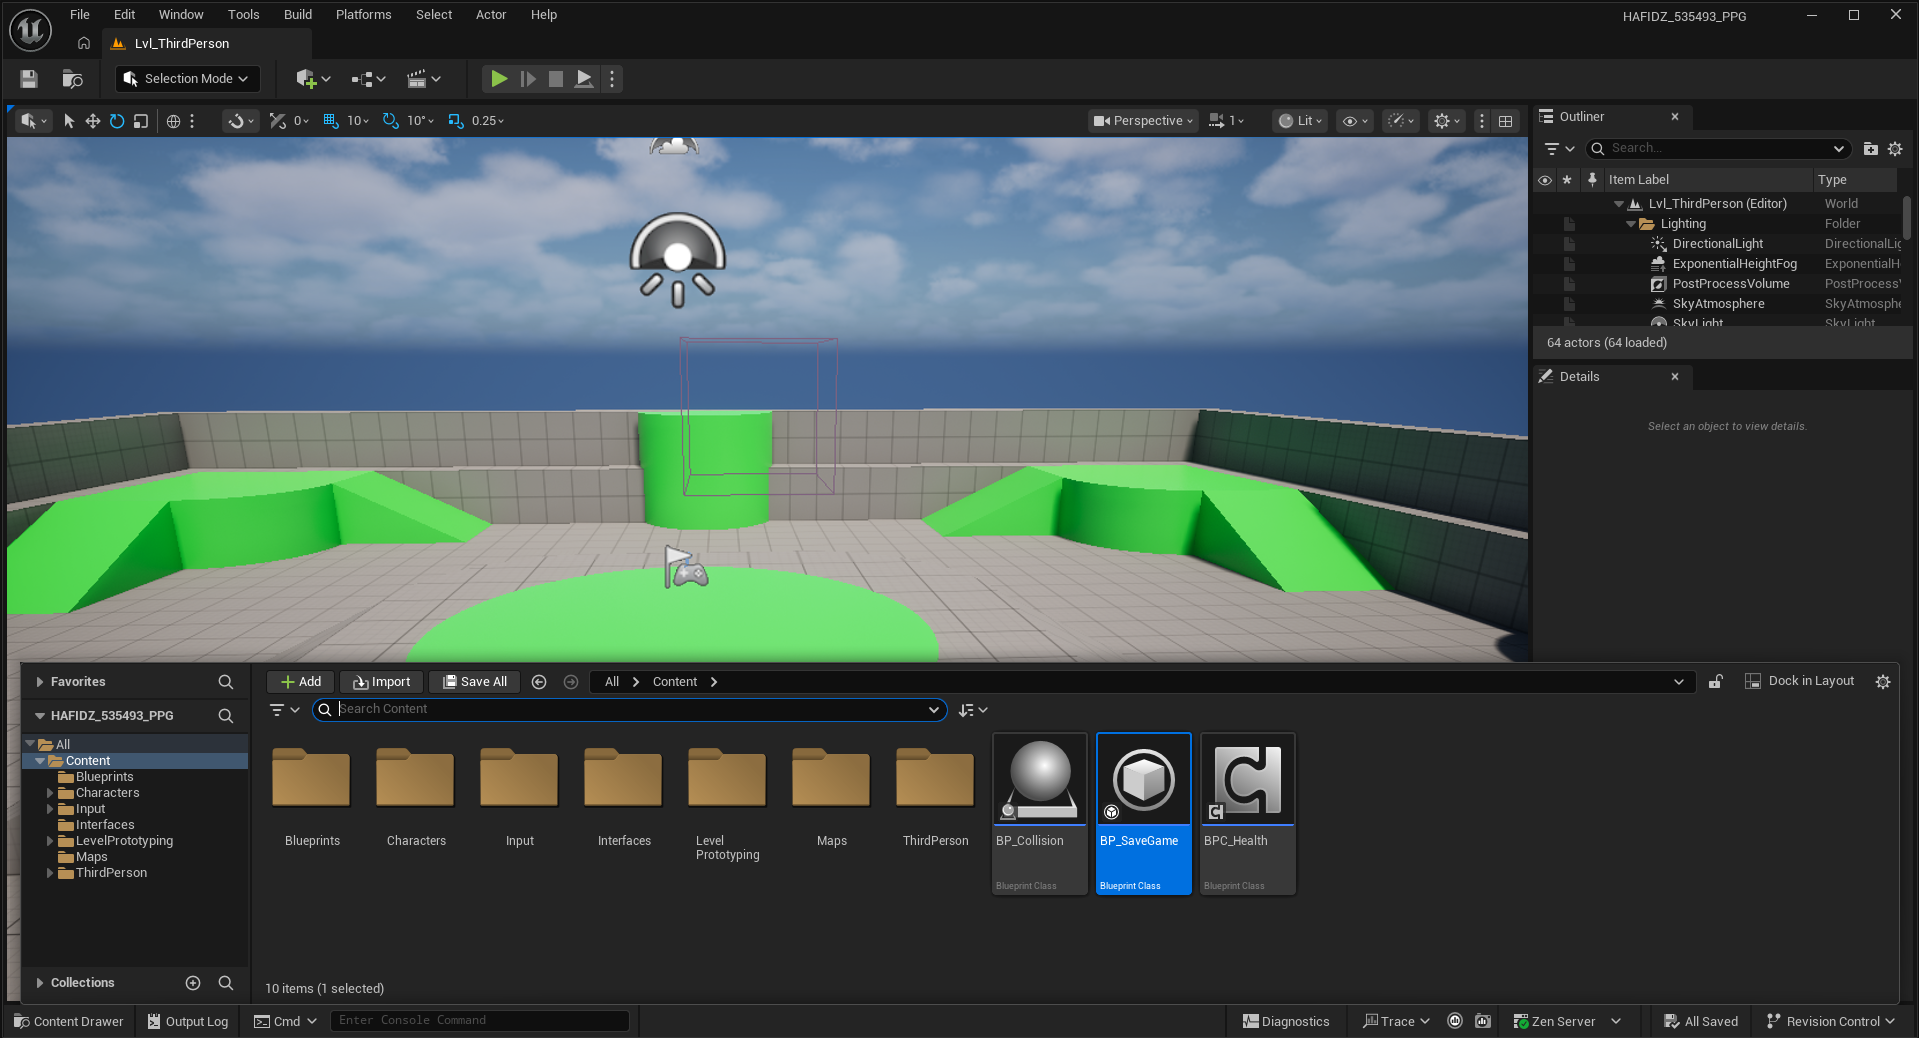
\includegraphics[width=0.9\textwidth]{images/ss-01-create-bp-savegame.png}}
    \caption{Pemilihan kelas induk SaveGame pada jendela Pick Parent Class untuk membuat aset BP\_SaveGame.}
    \label{fig:ss-create-bp-savegame}
\end{figure}

    \item \textbf{Pembuatan User Defined Structure (S\_PlayerState).} Pada Content Drawer, klik kanan dilakukan untuk membuka menu konteks \textbf{Blueprint > Structure}. Struktur data baru dibuat dan diberi nama \textbf{S\_PlayerState}. Tab editor struktur kemudian dibuka, dan satu variabel baru ditambahkan dengan nama \textbf{Transform} serta tipe data \textbf{Transform}. Konfigurasi ini menyatukan parameter lokasi, rotasi, dan skala karakter ke dalam satu kesatuan data.

\begin{figure}[H]
    \centering
    \customfbox{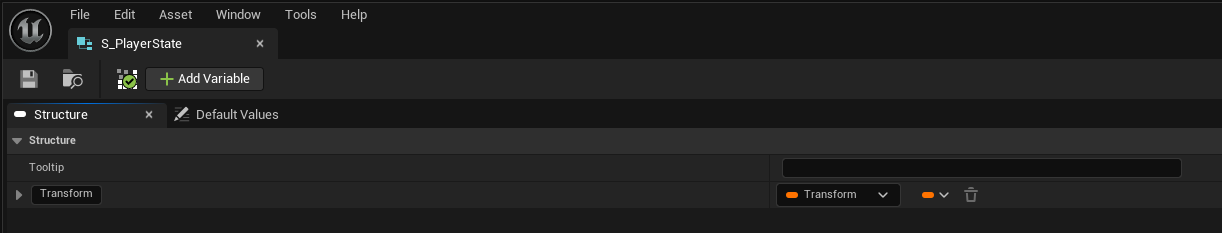
\includegraphics[width=0.9\textwidth]{images/ss-02-create-struct-playerstate.png}}
    \caption{Struktur data S\_PlayerState dengan variabel Transform bertipe data Transform.}
    \label{fig:ss-create-struct}
\end{figure}

    \item \textbf{Penambahan variabel struktur ke dalam BP\_SaveGame.} Berkas \texttt{BP\_SaveGame} dibuka pada editor Blueprint. Pada panel \textit{My Blueprint}, tombol tambah variabel ditekan untuk membuat variabel baru bernama \textbf{S\_PlayerState}. Tipe data variabel diatur mengarah ke struktur \textbf{S\_PlayerState} yang baru saja dibuat. Melalui langkah ini, berkas simpanan memiliki penampung untuk data posisi pemain.

\begin{figure}[H]
    \centering
    \customfbox{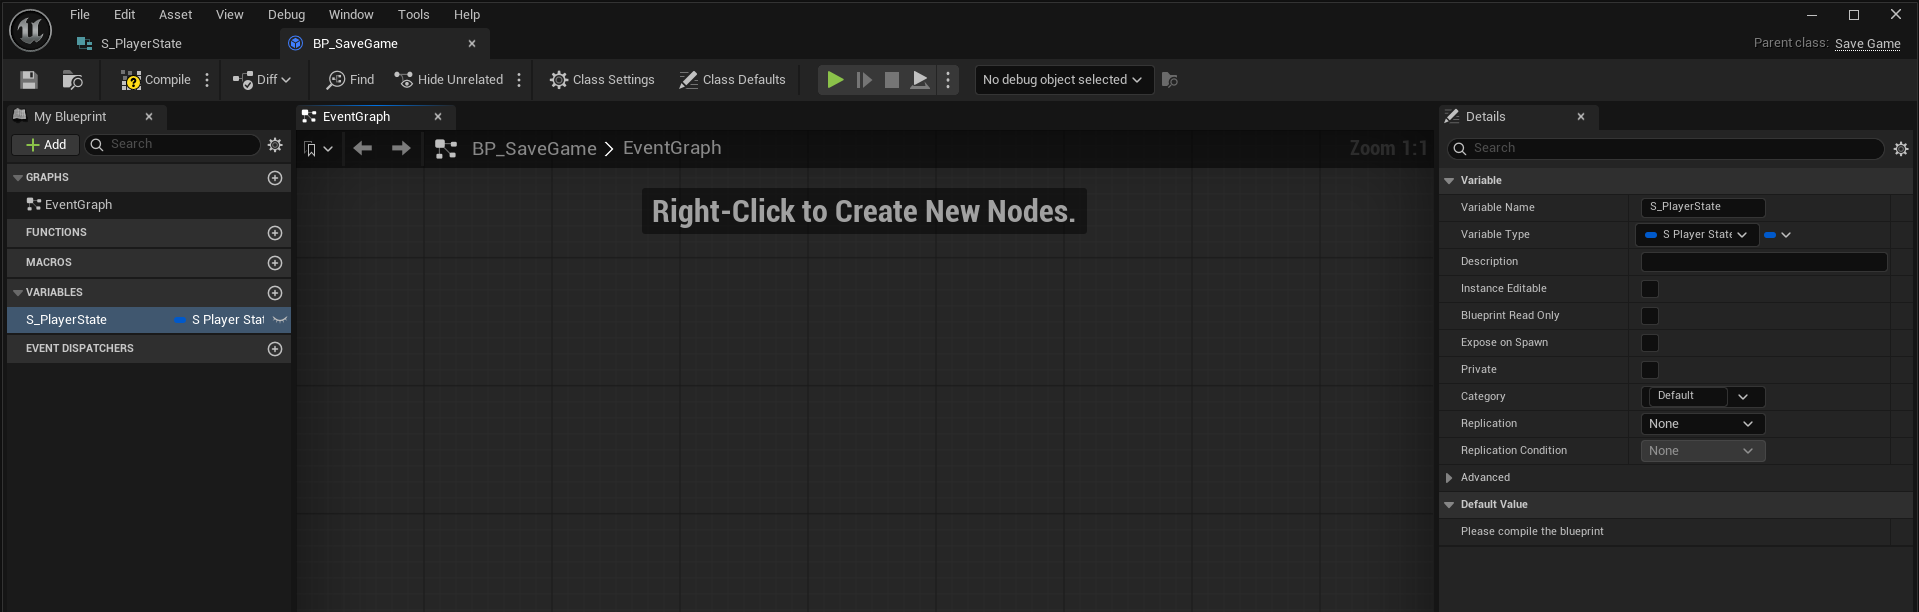
\includegraphics[width=0.9\textwidth]{images/ss-03-bp-savegame-variable.png}}
    \caption{Variabel S\_PlayerState bertipe data struktur S\_PlayerState pada panel My Blueprint BP\_SaveGame.}
    \label{fig:ss-savegame-variable}
\end{figure}
\end{enumerate}

\subsection{Konfigurasi Blueprint GameInstance pada Pengaturan Proyek}

\begin{enumerate}
    \item \textbf{Pembuatan BP\_GameInstance dan registrasi pada Project Settings.} Aset Blueprint baru dibuat dengan memilih kelas induk \textbf{GameInstance} dan dinamai \textbf{BP\_GameInstance}. Agar mesin game mengenali kelas ini sebagai pengelola instansi global utama, menu \textbf{Edit > Project Settings > Project - Maps \& Modes} dibuka. Pada seksi \textit{Game Instance}, opsi \textbf{Game Instance Class} diganti dari kelas bawaan mesin menjadi \textbf{BP\_GameInstance}.

\begin{figure}[H]
    \centering
    \customfbox{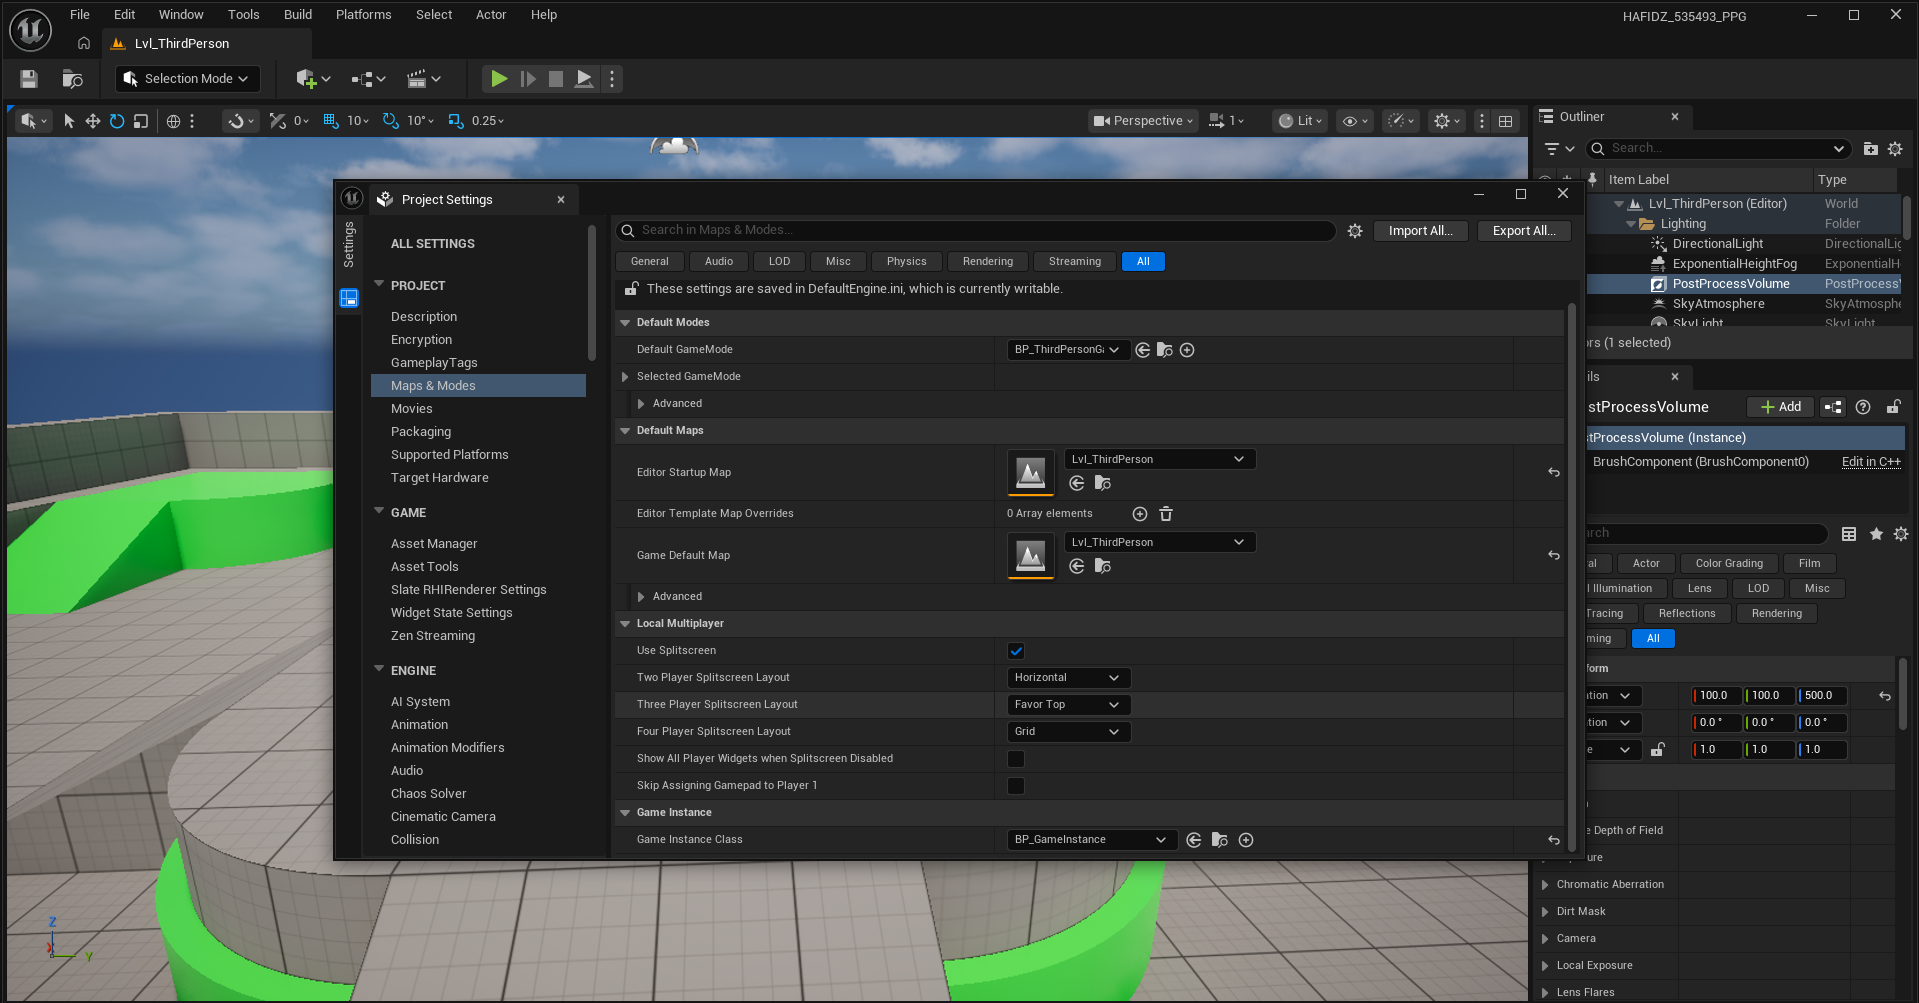
\includegraphics[width=0.9\textwidth]{images/ss-04-bp-gameinstance-project-settings.png}}
    \caption{Pembuatan BP\_GameInstance dan pengaturannya pada menu Project Settings bagian Maps \& Modes.}
    \label{fig:ss-gameinstance-settings}
\end{figure}

    \item \textbf{Deklarasi variabel SaveGame dan SlotName pada Game Instance.} Editor \texttt{BP\_GameInstance} dibuka. Dua variabel dibuat pada panel My Blueprint: variabel \textbf{SaveGame} bertipe referensi objek \textbf{BP\_SaveGame}, serta variabel \textbf{SlotName} bertipe data \textbf{String}. Pada panel Details variabel SlotName, nilai bawaan (\textit{Default Value}) diisi dengan string \texttt{"1"} sebagai pengenal slot berkas penyimpanan lokal.

\begin{figure}[H]
    \centering
    \customfbox{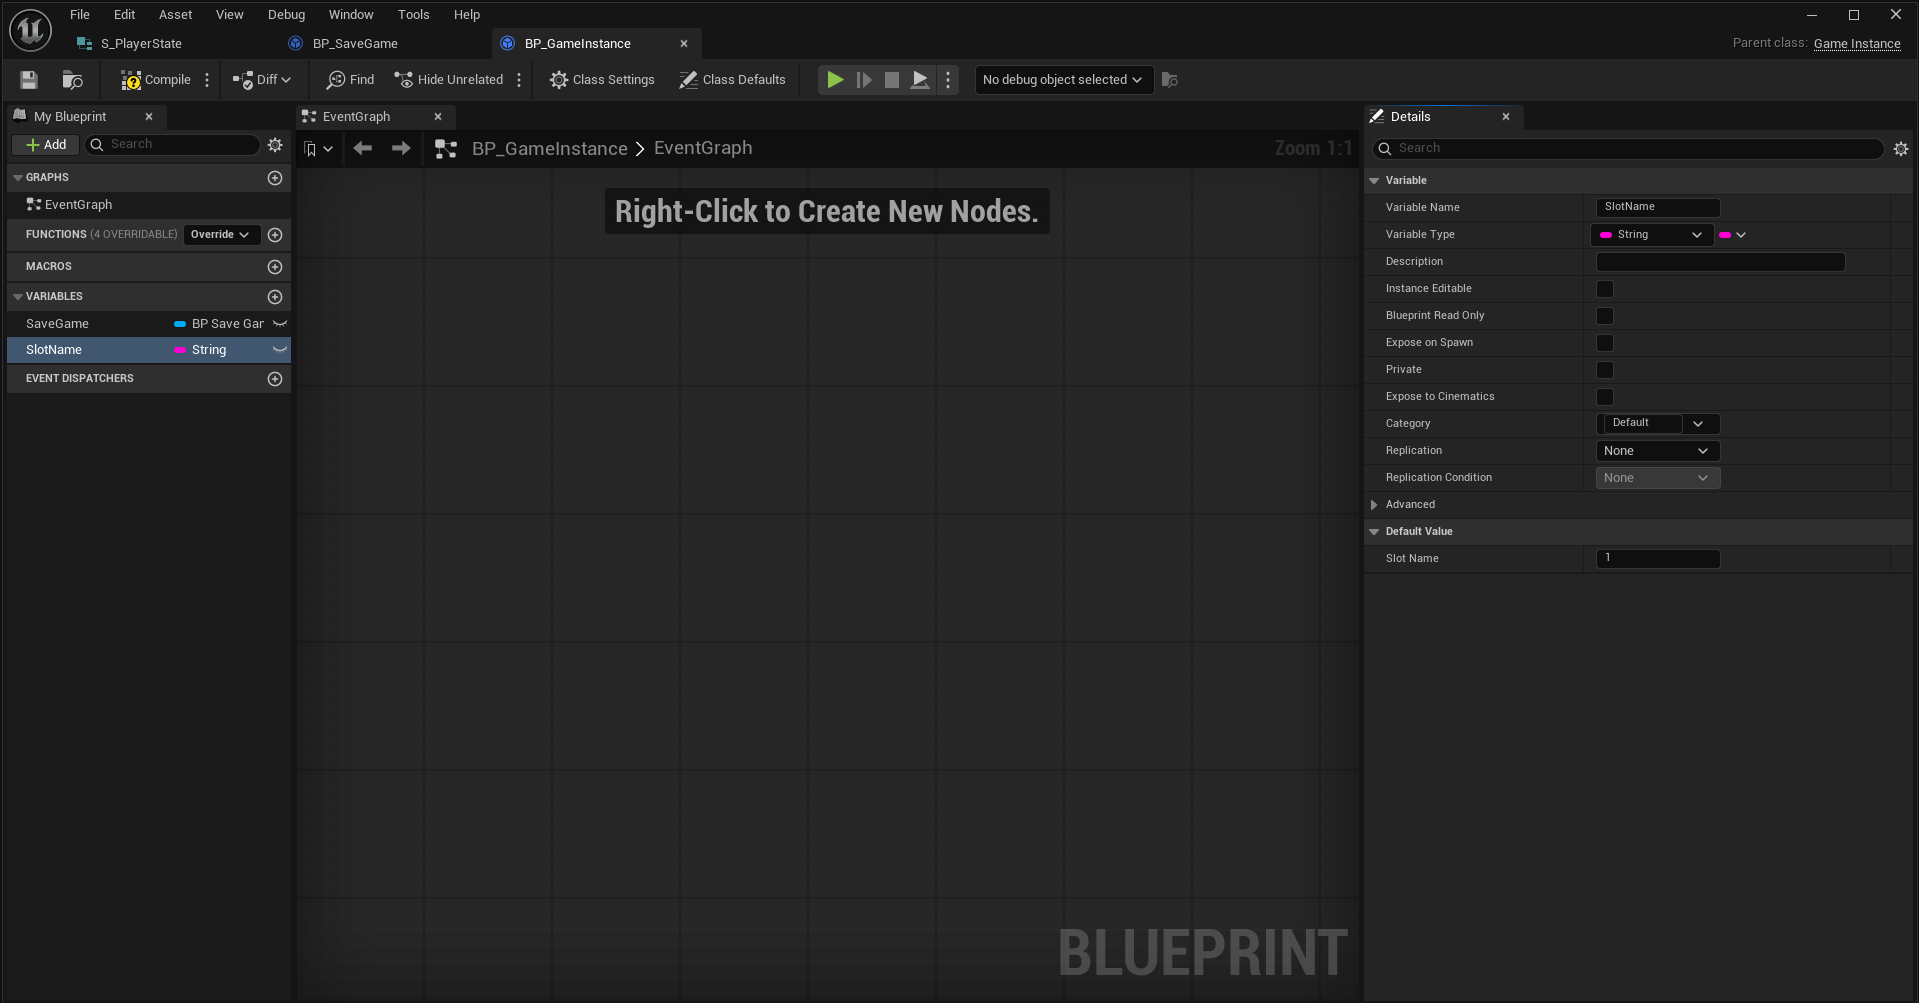
\includegraphics[width=0.9\textwidth]{images/ss-05-gameinstance-variables.png}}
    \caption{Panel variabel BP\_GameInstance yang memuat referensi objek SaveGame dan SlotName dengan nilai default 1.}
    \label{fig:ss-gameinstance-vars}
\end{figure}
\end{enumerate}

\subsection{Perancangan Blueprint Interface (BPI\_SaveData)}

\begin{enumerate}
    \item \textbf{Mendefinisikan fungsi dan parameter antarmuka BPI\_SaveData.} Pada direktori konten, aset Blueprint Interface dibuat dengan nama \textbf{BPI\_SaveData}. Empat fungsi operasional dideklarasikan di dalamnya beserta parameter masukan dan keluaran yang presisi:
    \begin{itemize}
        \item \textbf{LoadGameData}: memiliki parameter input \texttt{Async} bertipe Boolean.
        \item \textbf{SaveGameData}: memiliki parameter input \texttt{Async} bertipe Boolean.
        \item \textbf{GetGameData}: memiliki parameter output \texttt{S\_PlayerState} bertipe data struktur \texttt{S\_PlayerState}.
        \item \textbf{SavePlayer}: memiliki parameter input \texttt{S\_PlayerState} (tipe struktur \texttt{S\_PlayerState}) dan parameter input \texttt{Async} (tipe Boolean).
    \end{itemize}

\begin{figure}[H]
    \centering
    \customfbox{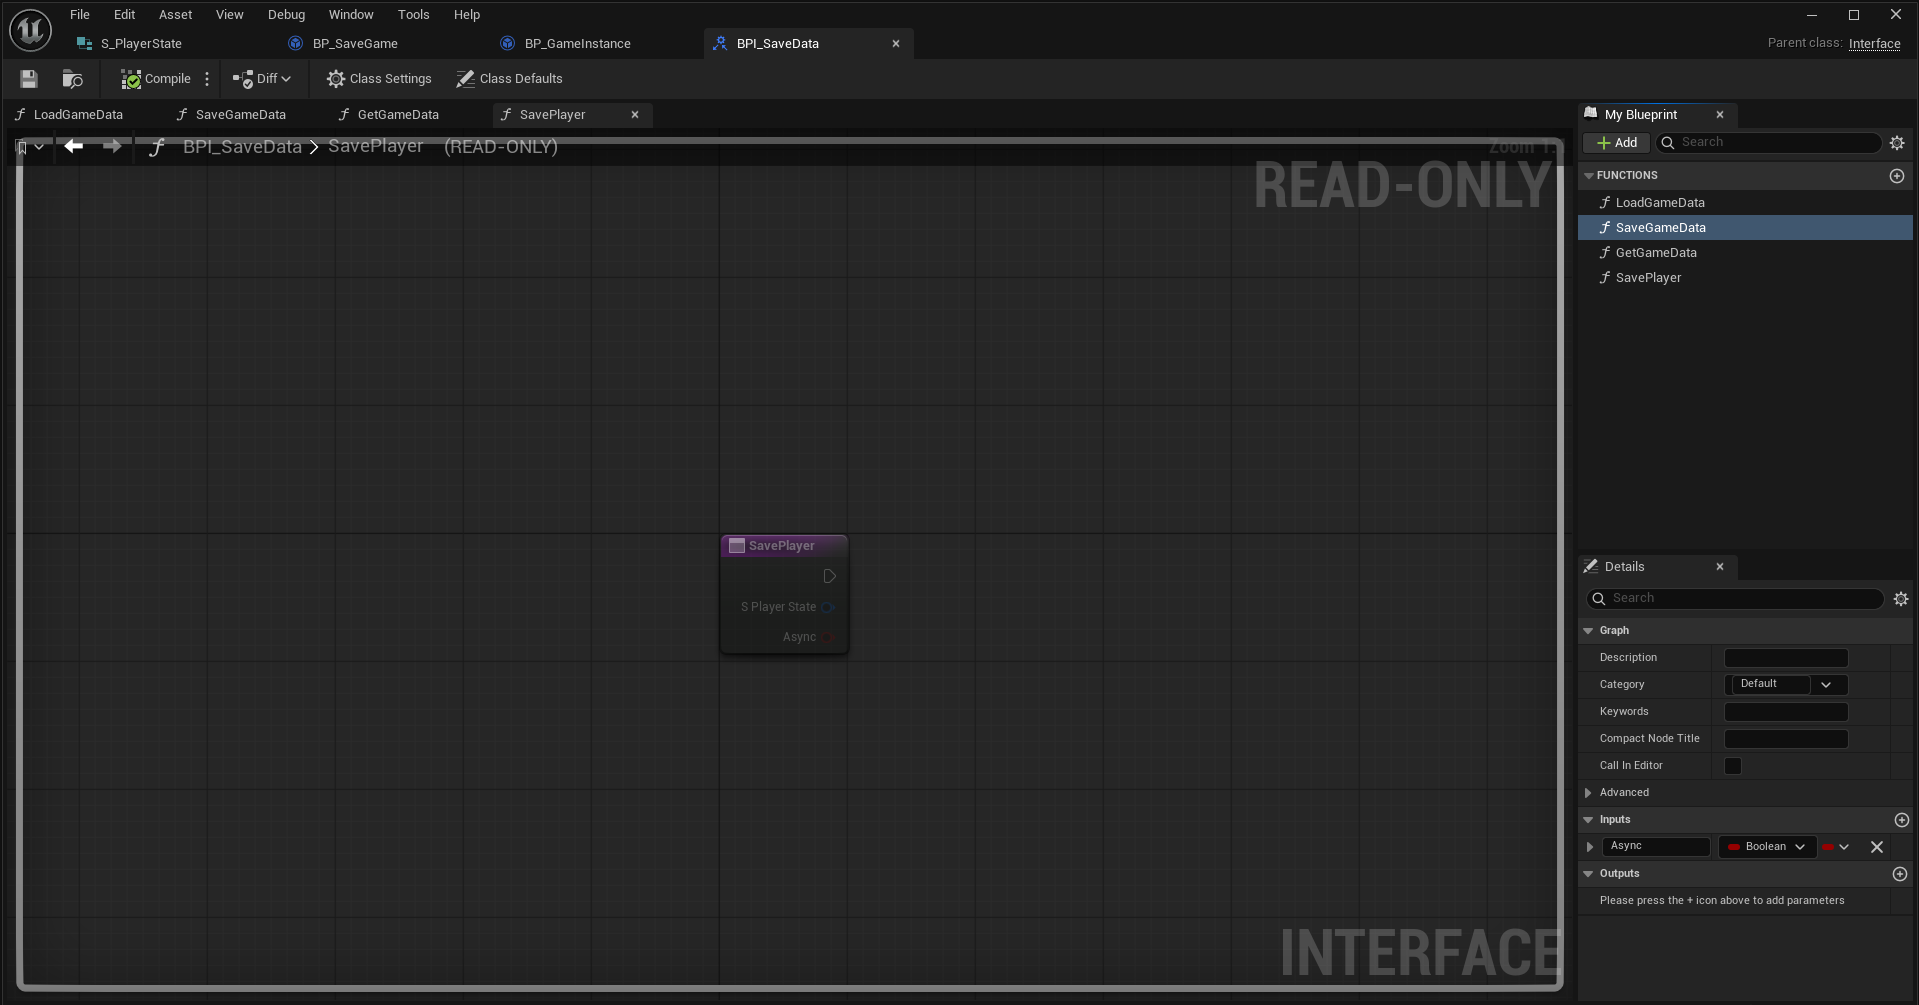
\includegraphics[width=0.9\textwidth]{images/ss-06-bpi-savedata-functions.png}}
    \caption{Daftar empat fungsi pada antarmuka BPI\_SaveData beserta konfigurasi parameter input dan output.}
    \label{fig:ss-bpi-functions}
\end{figure}
\end{enumerate}

\subsection{Implementasi Antarmuka pada BP\_GameInstance}

\begin{enumerate}
    \item \textbf{Penerapan BPI\_SaveData pada Class Settings.} Berkas \texttt{BP\_GameInstance} dibuka kembali, lalu tombol \textbf{Class Settings} pada toolbar atas diklik. Pada panel Details bagian \textbf{Interfaces > Implemented Interfaces}, tombol \textit{Add} ditekan untuk memasukkan \textbf{BPI\_SaveData}. Setelah Blueprint dikompilasi, keempat fungsi antarmuka muncul di bawah kategori \textbf{INTERFACES} pada panel My Blueprint.

\begin{figure}[H]
    \centering
    \customfbox{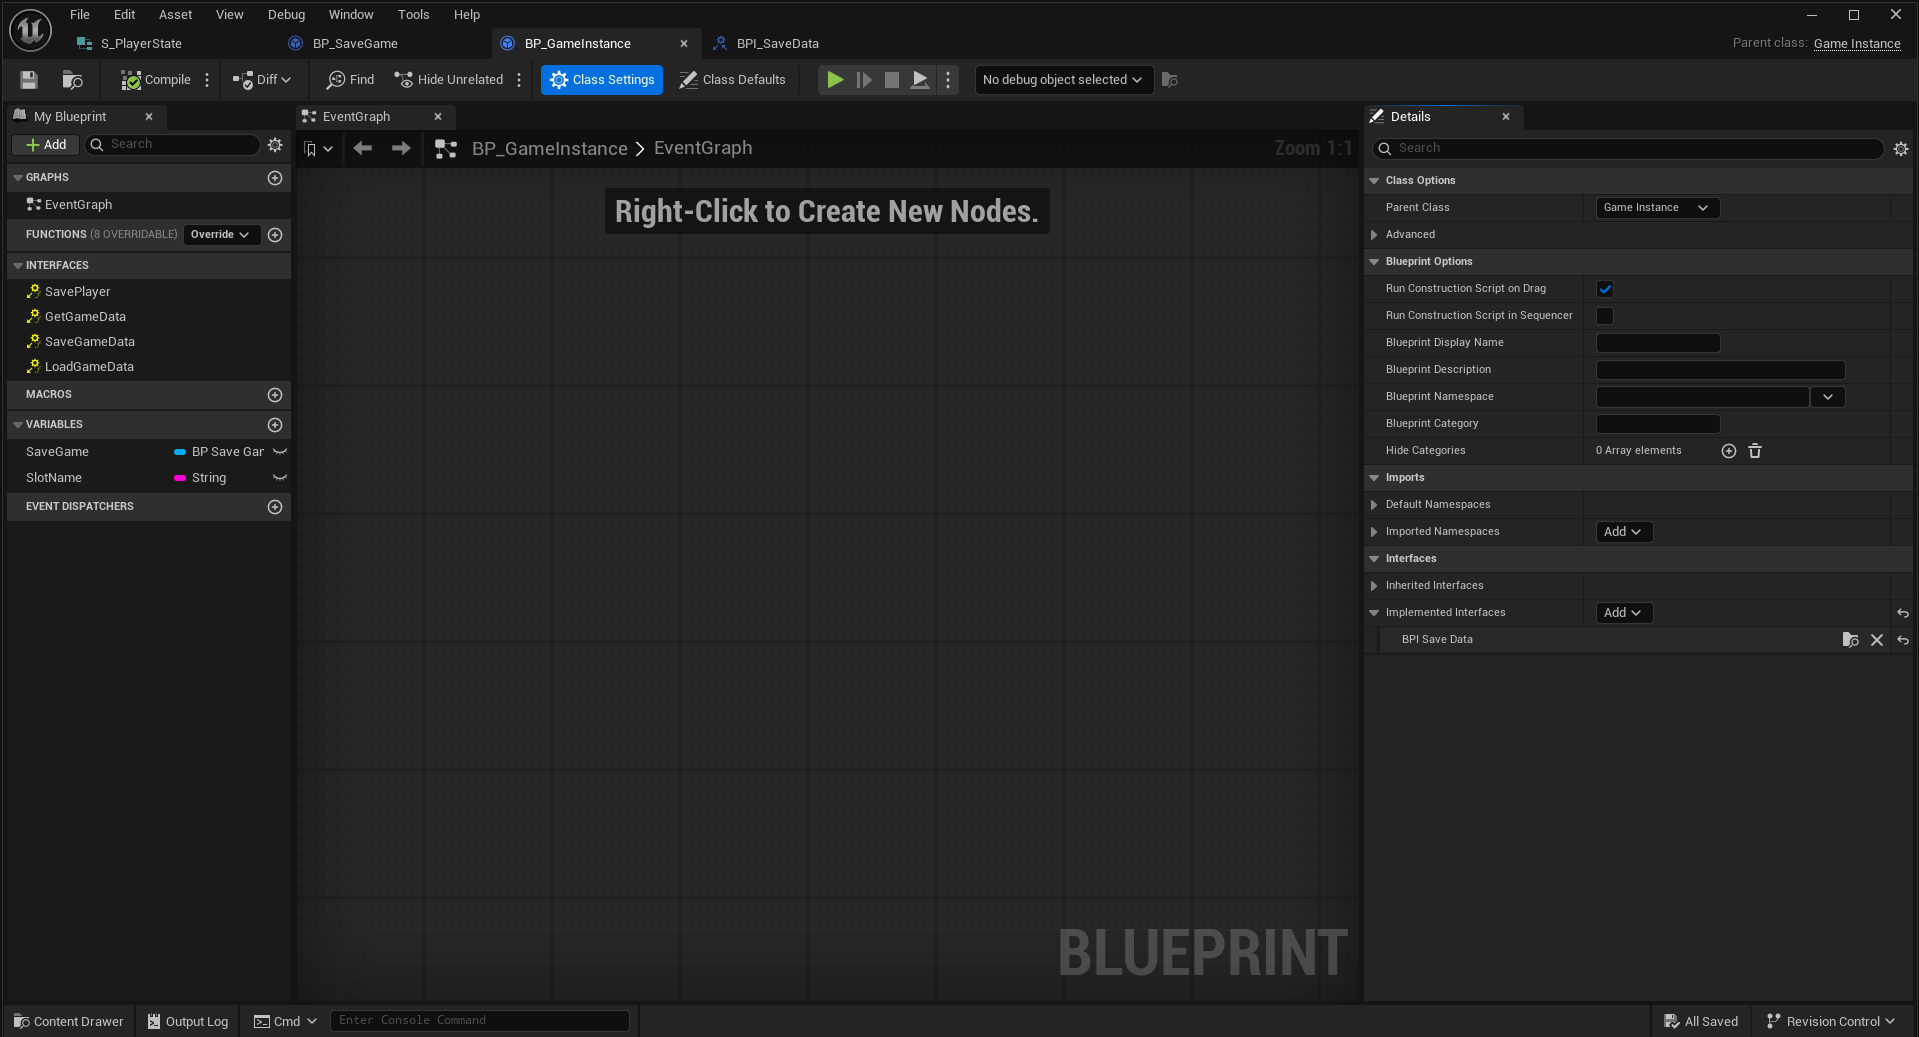
\includegraphics[width=0.9\textwidth]{images/ss-07-gameinstance-implement-interface.png}}
    \caption{Implementasi antarmuka BPI\_SaveData melalui Class Settings pada BP\_GameInstance.}
    \label{fig:ss-gameinstance-impl}
\end{figure}

    \item \textbf{Menyusun logika fungsi GetGameData.} Fungsi \texttt{GetGameData} dibuka untuk menyusun alur pengembalian data posisi. Node \textbf{Does Save Game Exist} dipasang dengan masukan \texttt{SlotName} dan \texttt{User Index 0} untuk memeriksa keberadaan berkas di penyimpanan. Hasil pemeriksaan disambungkan ke node \textbf{Branch}. Jika bernilai benar (True), nilai \texttt{S\_PlayerState} diambil dari variabel \texttt{SaveGame} dan dikembalikan melalui \textbf{Return Node}. Jika salah (False), Return Node mengembalikan koordinat default dengan posisi (0, 0, 0) dan skala (1, 1, 1).

\begin{figure}[H]
    \centering
    \customfbox{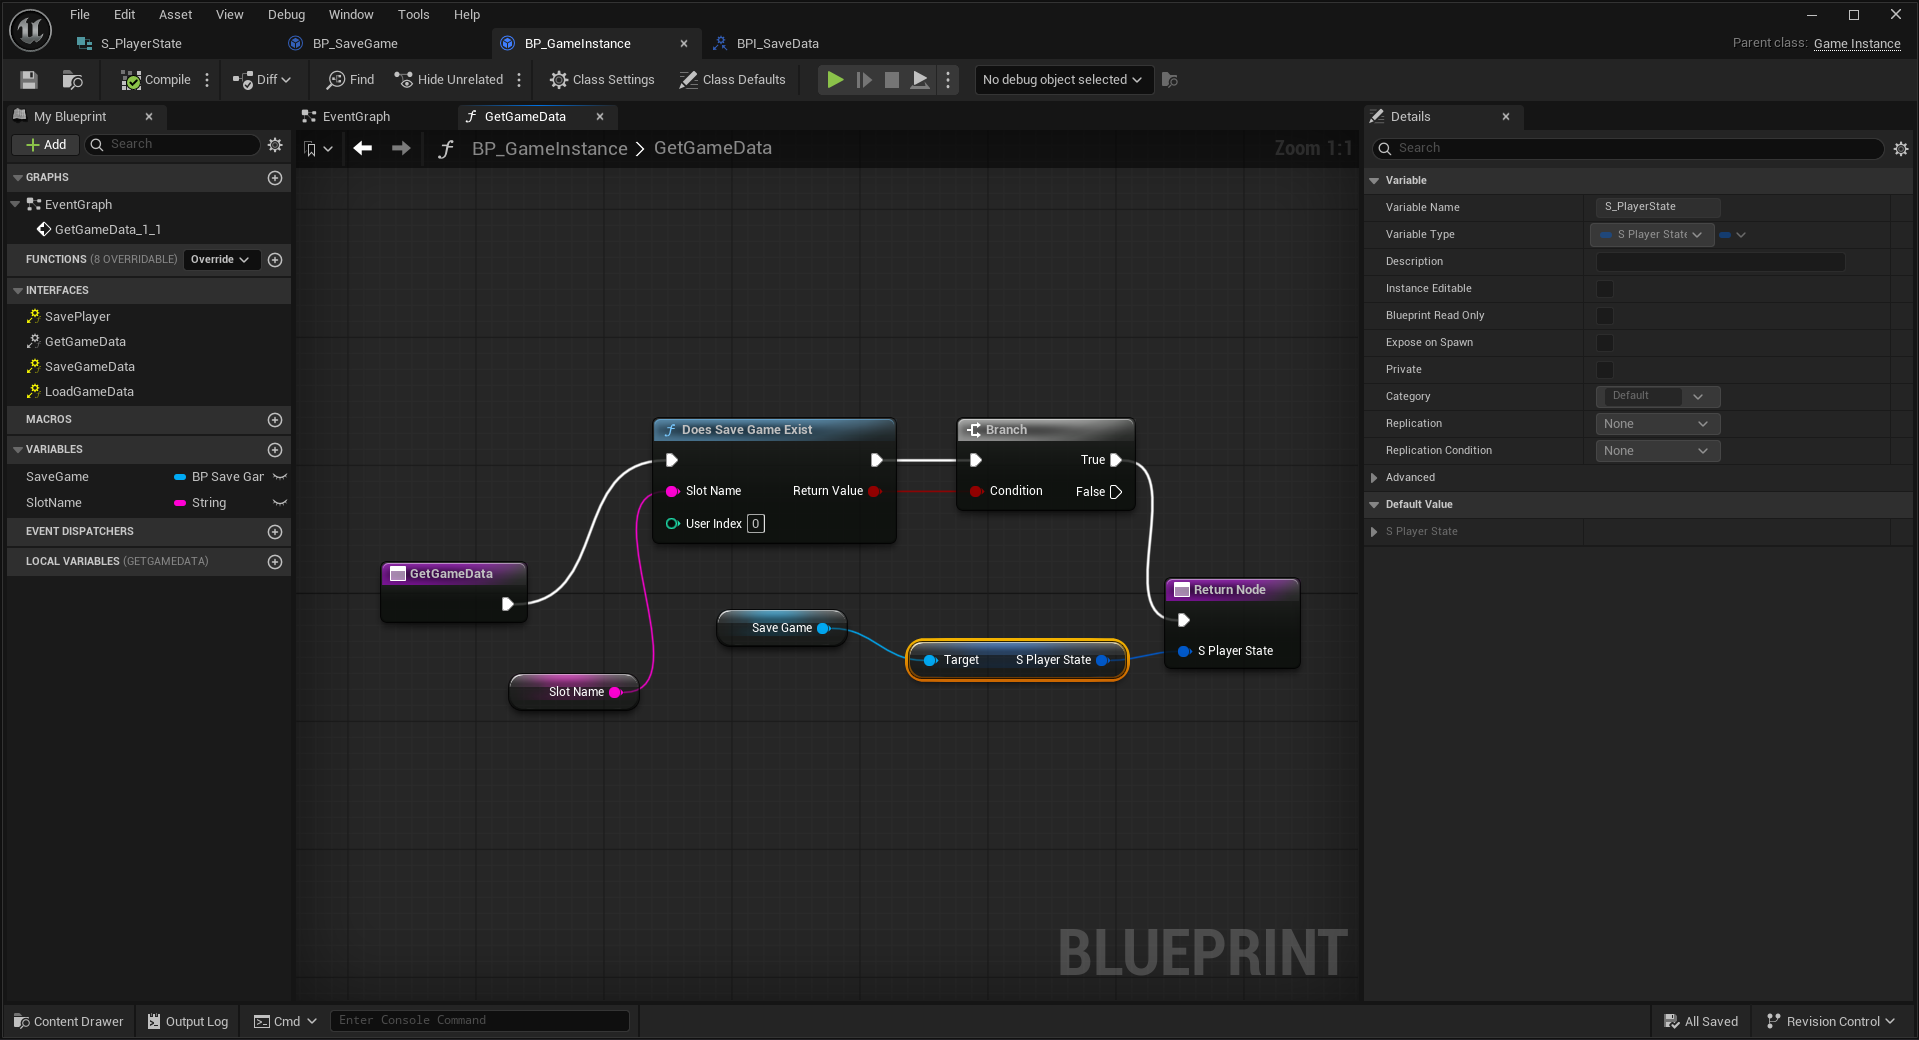
\includegraphics[width=0.9\textwidth]{images/ss-08-gameinstance-getgamedata.png}}
    \caption{Rangkaian graph fungsi GetGameData: validasi keberadaan berkas simpanan dan pengembalian data posisi.}
    \label{fig:ss-func-getgamedata}
\end{figure}

    \item \textbf{Menyusun logika fungsi SavePlayer.} Fungsi \texttt{SavePlayer} dibuka untuk menerima data terbaru karakter. Node event menerima struktur \texttt{S\_PlayerState} dan boolean \texttt{Async}. Alur graph mengeksekusi node \textbf{SET S\_PlayerState} pada objek variabel \texttt{SaveGame} yang ada di memori. Selanjutnya, alur diteruskan untuk memanggil fungsi \textbf{SaveGameData} dengan membawa nilai boolean Async tersebut.

\begin{figure}[H]
    \centering
    \customfbox{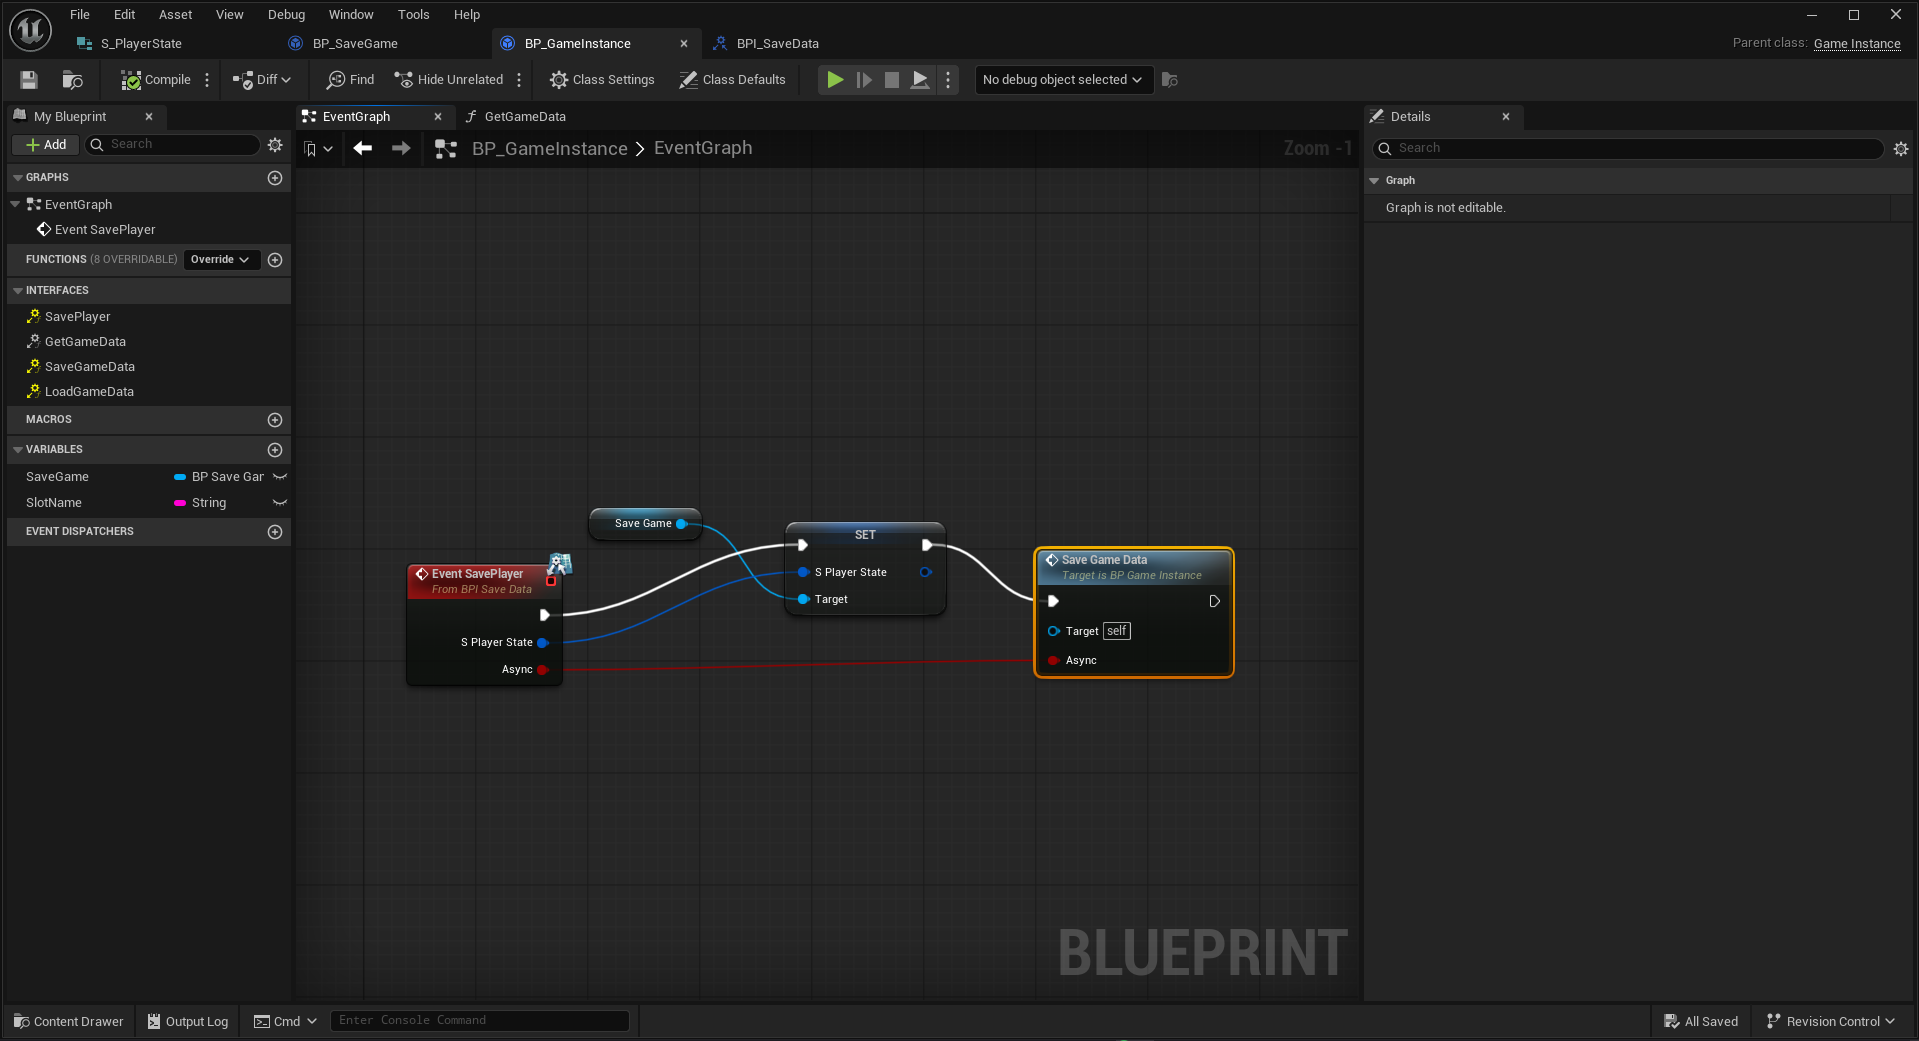
\includegraphics[width=0.9\textwidth]{images/ss-09-gameinstance-saveplayer.png}}
    \caption{Graph fungsi SavePlayer: memperbarui nilai struktur pada objek SaveGame lalu memanggil fungsi SaveGameData.}
    \label{fig:ss-func-saveplayer}
\end{figure}

    \item \textbf{Menyusun logika fungsi SaveGameData.} Logika fungsi \texttt{SaveGameData} dibuka untuk menangani proses penulisan ke media penyimpanan lokal. Parameter boolean \texttt{Async} disambungkan ke node \textbf{Branch}. Jika True, node \textbf{Async Save Game to Slot} dipanggil menggunakan masukan objek \texttt{SaveGame} dan \texttt{SlotName}. Jika False, penyimpanan dieksekusi secara sinkron melalui node standar \textbf{Save Game to Slot}.

\begin{figure}[H]
    \centering
    \customfbox{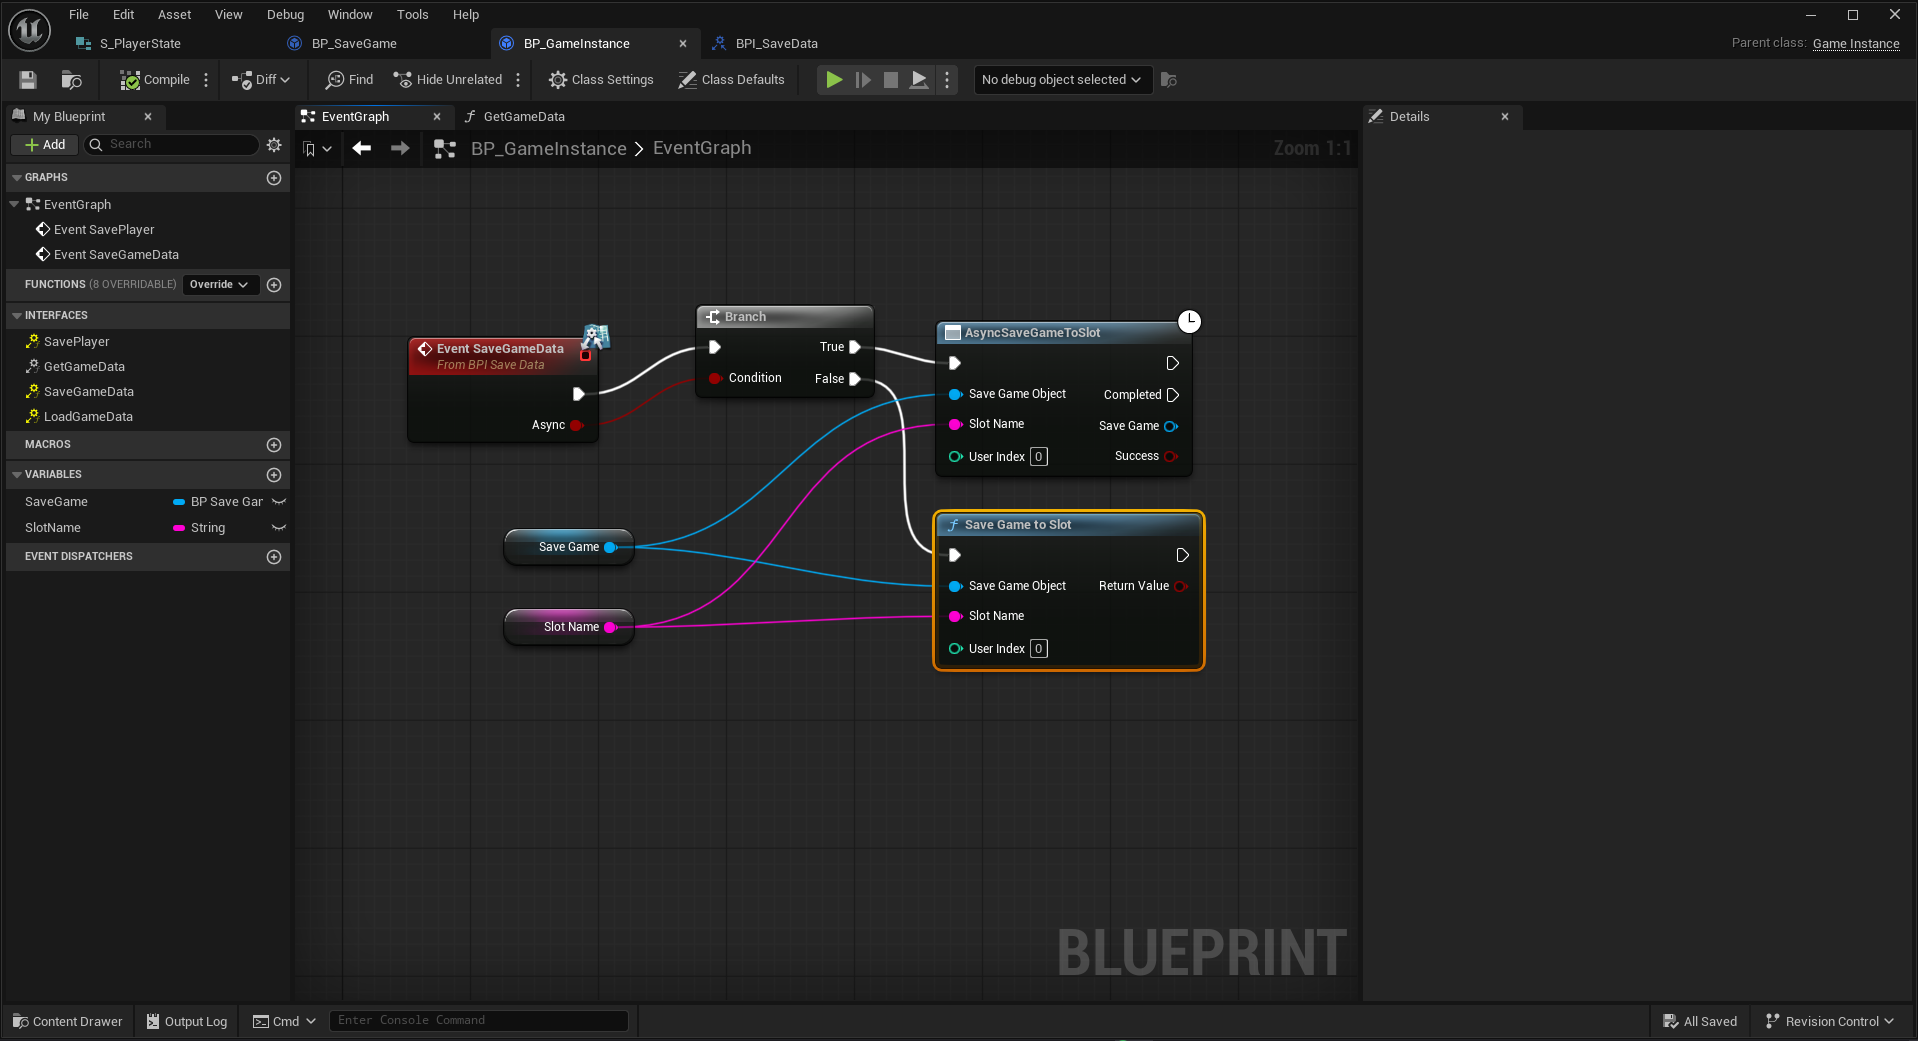
\includegraphics[width=0.9\textwidth]{images/ss-10-gameinstance-savegamedata.png}}
    \caption{Graph fungsi SaveGameData: percabangan penyimpanan berkas mode asinkron atau sinkron ke slot.}
    \label{fig:ss-func-savegamedata}
\end{figure}

    \item \textbf{Menyusun logika fungsi LoadGameData.} Logika fungsi \texttt{LoadGameData} bertugas memuat berkas simpanan ke memori RAM. Graph diawali dengan memeriksa keberadaan berkas menggunakan \textbf{Does Save Game Exist}. Jika berkas ada (True), percabangan memeriksa opsi Async untuk memanggil \textbf{Async Load Game from Slot} atau \textbf{Load Game from Slot}. Objek hasil pemuatan di-cast ke \textbf{BP\_Savegame} lalu disimpan ke variabel \texttt{SaveGame}. Jika berkas belum ditemukan (False), alur memanggil node \textbf{Create Save Game Object} dari kelas \texttt{BP\_SaveGame} dan menetapkannya ke variabel \texttt{SaveGame} sebagai data awal.

\begin{figure}[H]
    \centering
    \customfbox{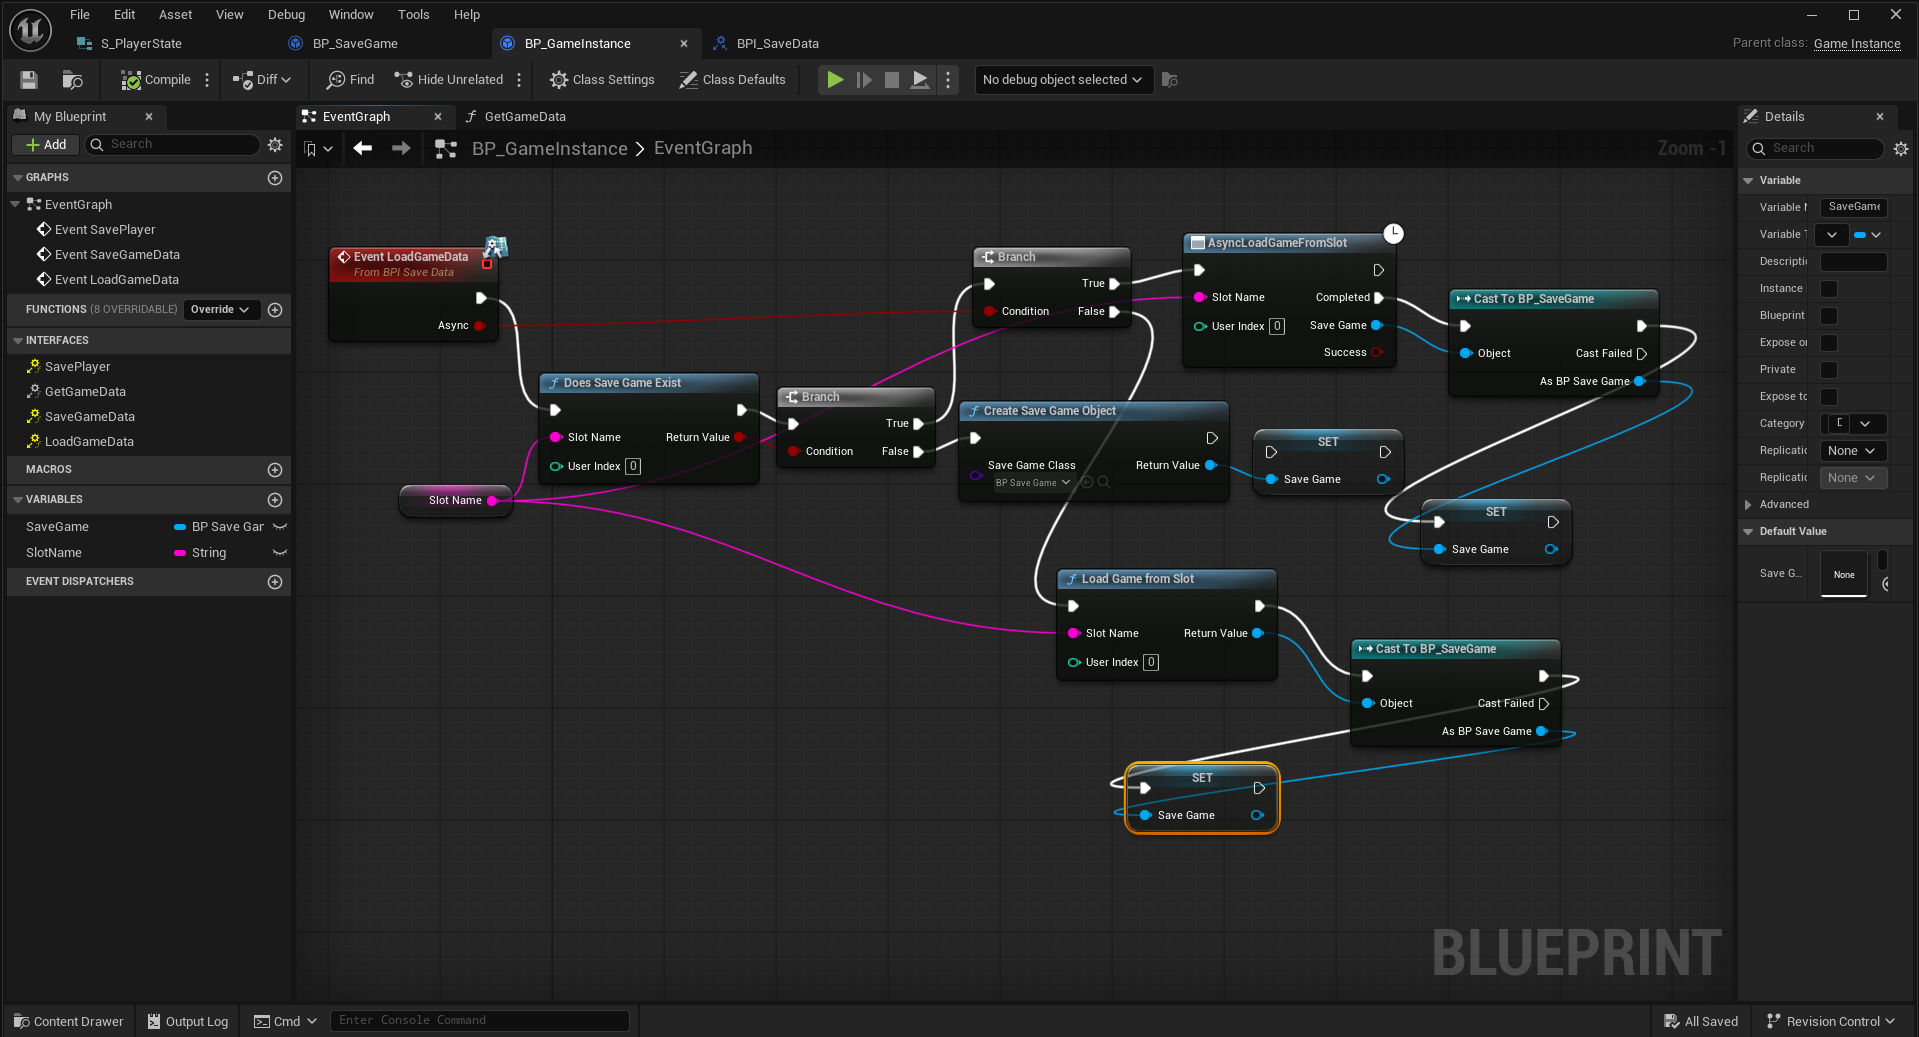
\includegraphics[width=0.9\textwidth]{images/ss-11-gameinstance-loadgamedata.png}}
    \caption{Graph fungsi LoadGameData: pembacaan berkas dari disk atau pembuatan objek simpanan baru jika belum ada.}
    \label{fig:ss-func-loadgamedata}
\end{figure}
\end{enumerate}

\subsection{Inisialisasi Data pada Event Init GameInstance}

\begin{enumerate}
    \item \textbf{Menghubungkan Event Init ke pemanggilan LoadGameData.} Pada Event Graph utama milik \texttt{BP\_GameInstance}, node \textbf{Event Init} diletakkan. Pin eksekusi Event Init disambungkan langsung ke pemanggilan fungsi \textbf{Load Game Data} dengan target \textit{self} dan parameter Async dibiarkan nonaktif. Pengaturan ini memastikan berkas simpanan langsung dibaca saat game pertama kali dibuka sebelum level dan aktor dimuat.

\begin{figure}[H]
    \centering
    \customfbox{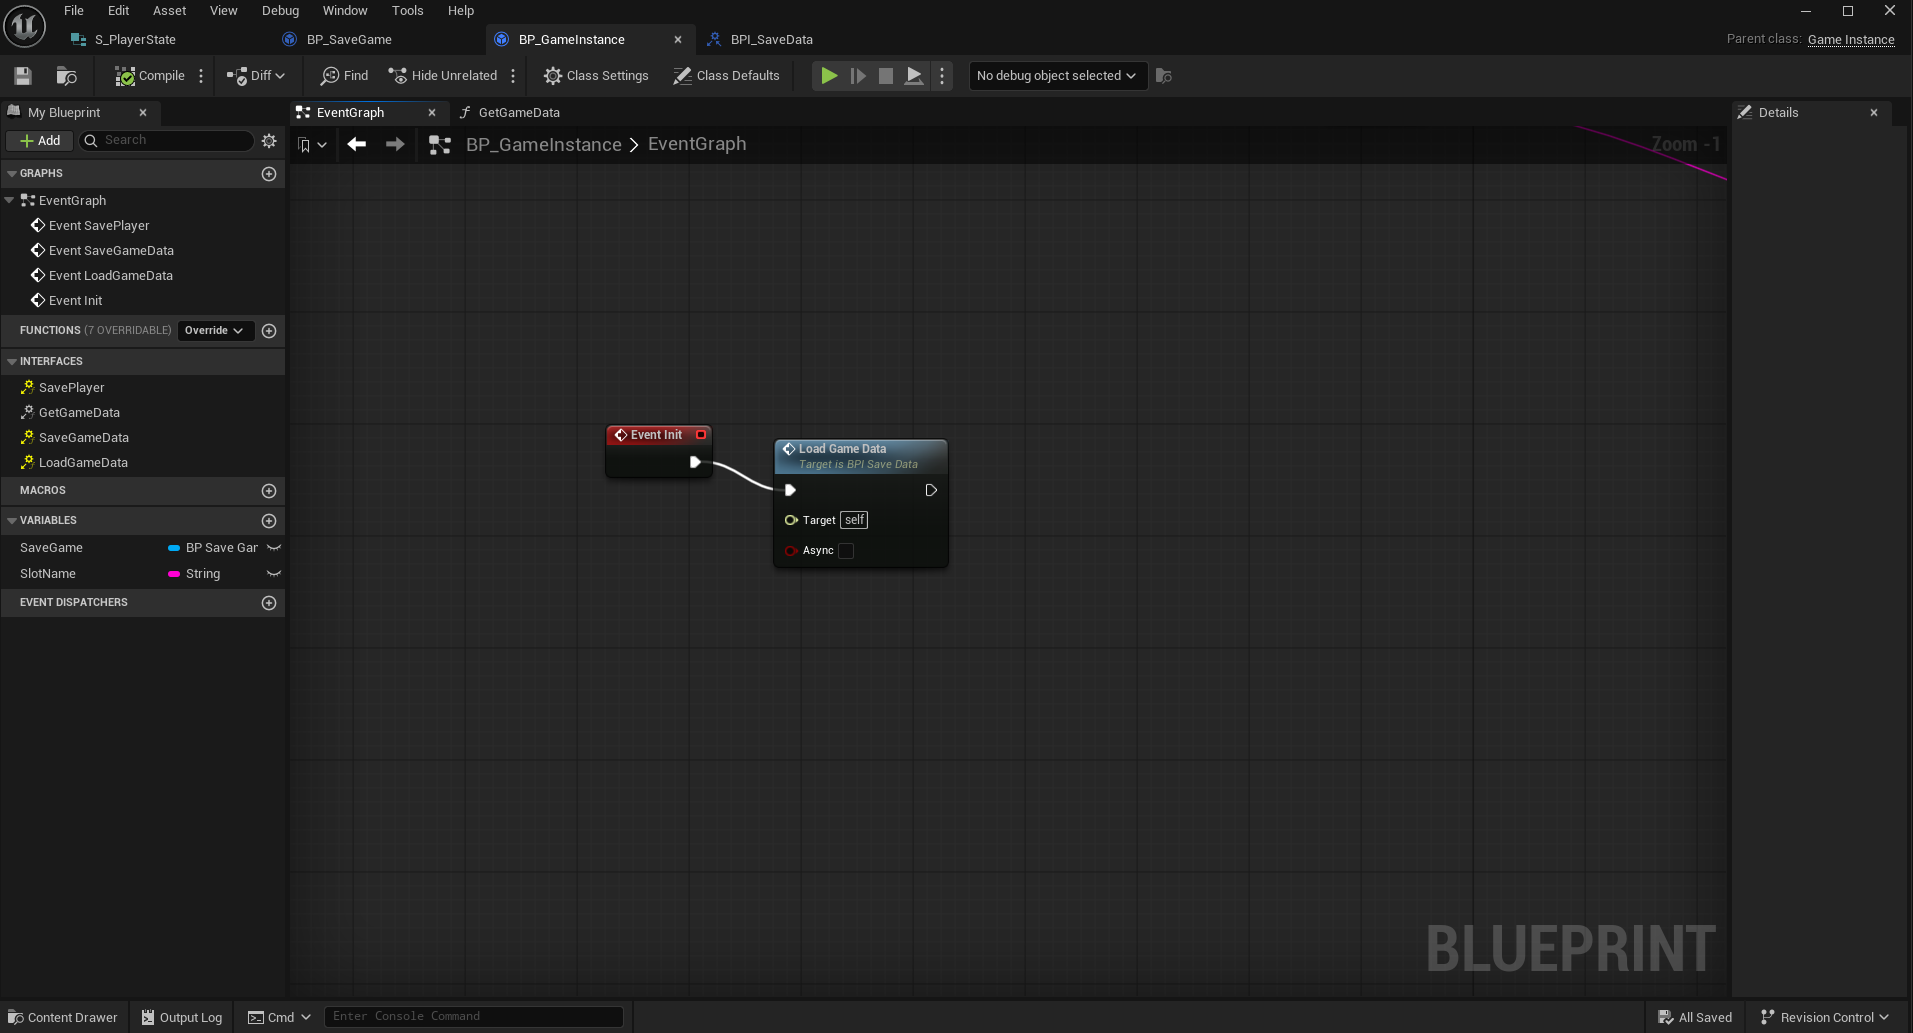
\includegraphics[width=0.9\textwidth]{images/ss-12-gameinstance-event-init.png}}
    \caption{Eksekusi pemuatan data awal melalui Event Init pada Event Graph BP\_GameInstance.}
    \label{fig:ss-event-init}
\end{figure}
\end{enumerate}

\subsection{Pemulihan Posisi Karakter pada BP\_ThirdPersonCharacter}

\begin{enumerate}
    \item \textbf{Membaca data simpanan dan memperbarui posisi pada BeginPlay.} Karakter \texttt{BP\_ThirdPersonCharacter} dibuka pada editor Blueprint. Pada Event Graph, node \textbf{Event BeginPlay} disambungkan ke node panggilan pesan antarmuka \textbf{Get Game Data} dengan target dari node \textbf{Get Game Instance}. Struktur keluaran diurai untuk mengambil nilai koordinat lokasi. Sebuah node \textbf{Branch} memeriksa apakah koordinat lokasi tidak bernilai nol (0, 0, 0). Jika True, node \textbf{Set Actor Location} dijalankan untuk memindahkan karakter ke posisi simpanan tersebut.

\begin{figure}[H]
    \centering
    \customfbox{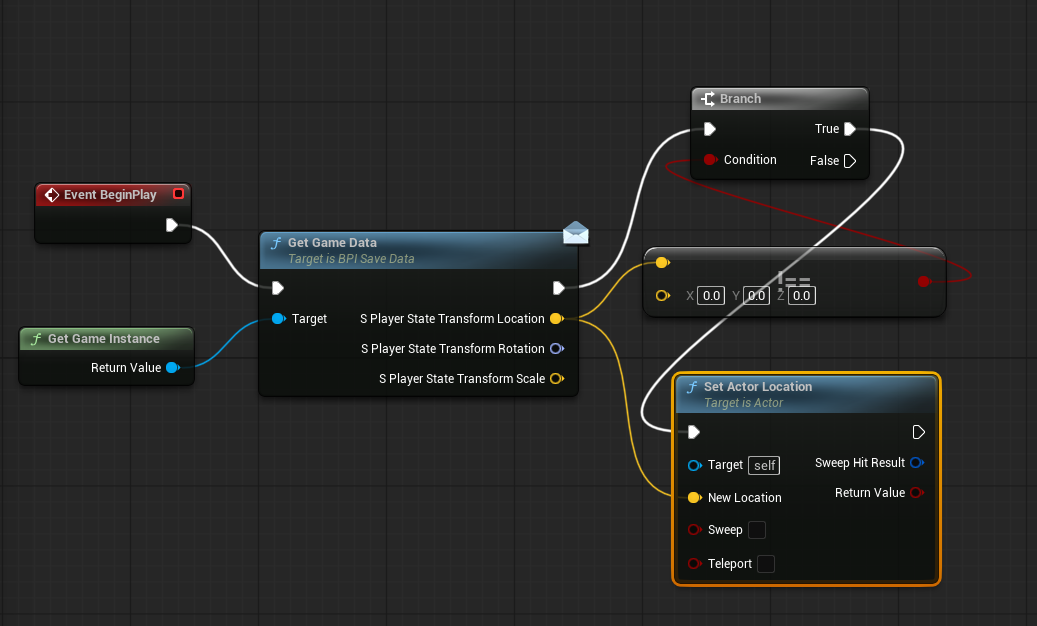
\includegraphics[width=0.9\textwidth]{images/ss-13-character-beginplay-restore-location.png}}
    \caption{Logika BeginPlay pada karakter pemain untuk memulihkan koordinat lokasi dari Game Instance.}
    \label{fig:ss-char-beginplay}
\end{figure}
\end{enumerate}

\subsection{Perancangan Aktor Pemicu Checkpoint (BP\_CheckPoint)}

\begin{enumerate}
    \item \textbf{Merancang komponen dan logika pemicu pada BP\_CheckPoint.} Aktor Blueprint baru dibuat dengan nama \textbf{BP\_CheckPoint}. Di dalam hierarki komponen, komponen \textbf{Box Collision} bernama \texttt{Box} ditambahkan. Pada Event Graph, event \textbf{On Component Begin Overlap (Box)} disambungkan ke node \textbf{Do Once} agar pencatatan hanya terjadi satu kali saat dilewati. Selanjutnya, node \textbf{Get Actor Transform} mengambil posisi checkpoint, dan node \textbf{Get Game Instance} menjadi target panggilan pesan antarmuka \textbf{Save Player} dengan opsi Async diaktifkan.

\begin{figure}[H]
    \centering
    \customfbox{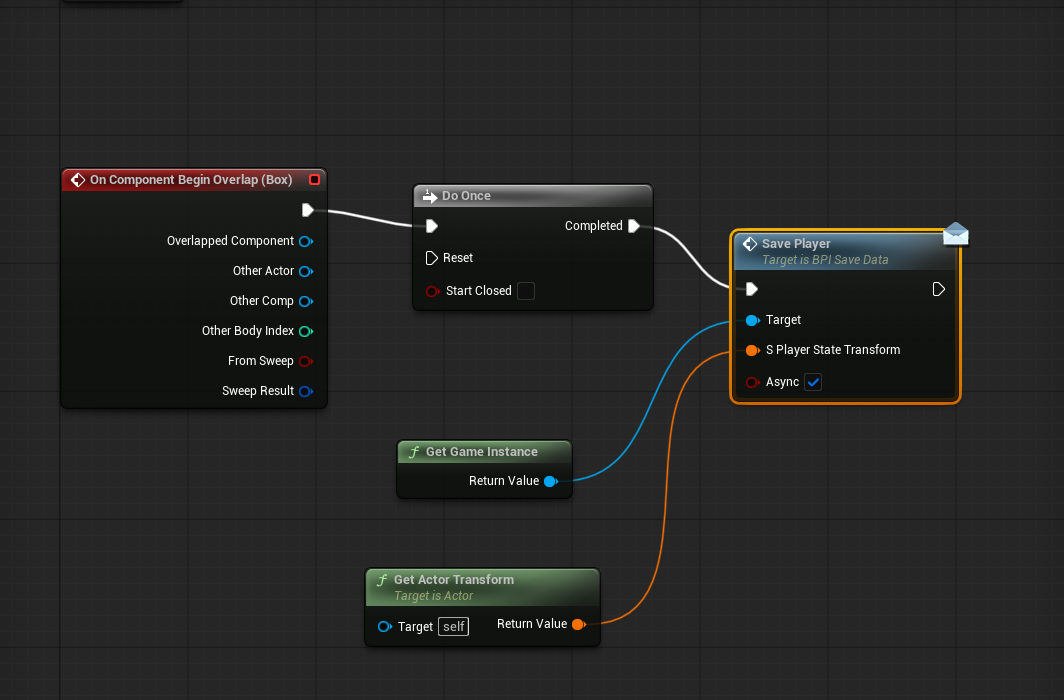
\includegraphics[width=0.9\textwidth]{images/ss-14-create-bp-checkpoint.png}}
    \caption{Komponen Box Collision dan alur Overlap pada BP\_CheckPoint yang memanggil interface Save Player.}
    \label{fig:ss-bp-checkpoint}
\end{figure}

    \item \textbf{Menempatkan instance BP\_CheckPoint pada level.} Aktor \texttt{BP\_CheckPoint} diseret dari Content Drawer ke dalam viewport level permainan. Checkpoint diletakkan di tengah lintasan pada posisi koordinat tertentu di depan area awal pemain (\texttt{PlayerStart}) agar dapat dilalui secara langsung oleh karakter saat berjalan.

\begin{figure}[H]
    \centering
    \customfbox{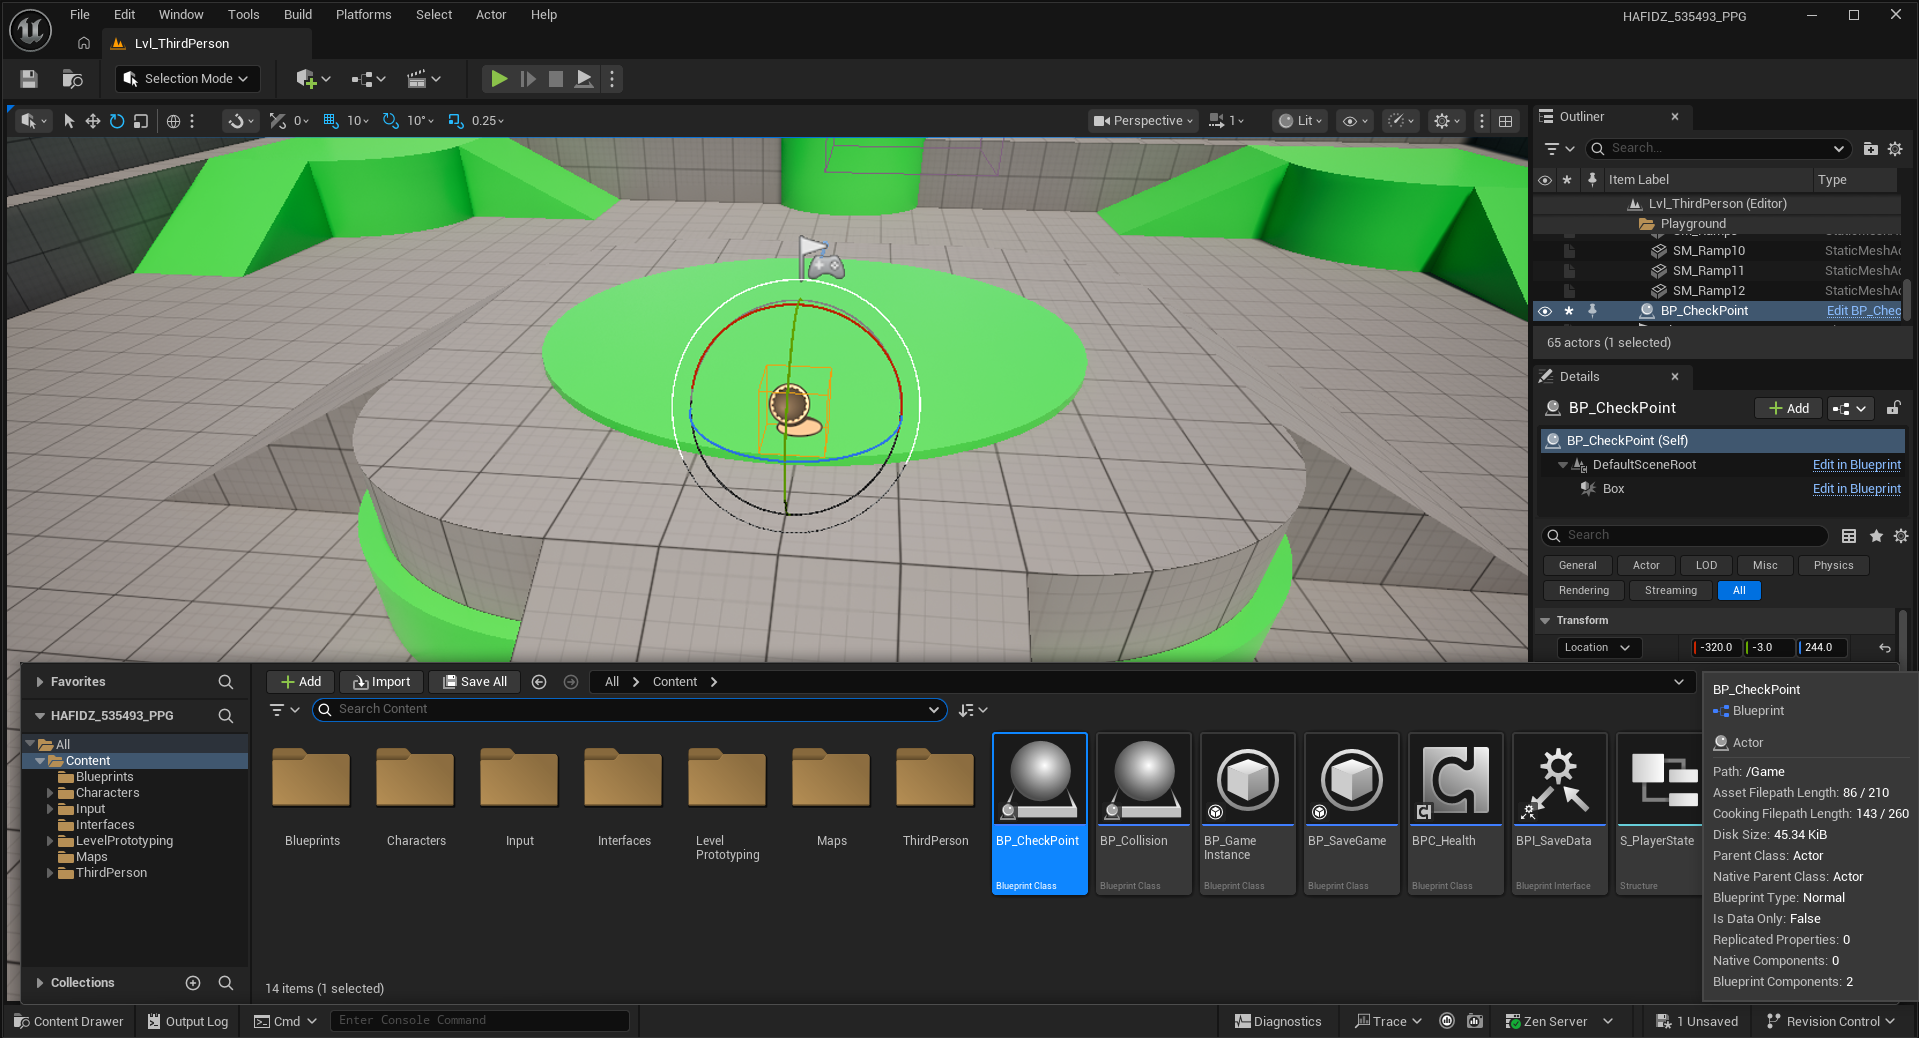
\includegraphics[width=0.9\textwidth]{images/ss-15-placement-checkpoint-in-level.png}}
    \caption{Penempatan instance aktor BP\_CheckPoint pada viewport level permainan.}
    \label{fig:ss-level-placement}
\end{figure}
\end{enumerate}

\section{Hasil Akhir}
Pengujian sistem dilakukan langsung di dalam editor level Unreal Engine 5.8 dengan menekan tombol \textbf{Play}. Pada tahap awal pengujian, karakter Third Person muncul di titik awal standar yang ditentukan oleh aktor \texttt{PlayerStart}. Karakter kemudian digerakkan melintasi rintangan menuju ke arah volume kawat \texttt{BP\_CheckPoint}. Saat karakter menyentuh batas tabrakan, event overlap terpicu. Node \texttt{Do Once} memastikan event hanya ditembakkan satu kali, mengambil koordinat transform tempat karakter berada, lalu mengirimkan data tersebut ke Game Instance melalui fungsi pesan \texttt{Save Player} secara asinkron. Berkas \texttt{1.sav} berhasil diperbarui di media penyimpanan lokal tanpa ada penurunan kestabilan visual pada viewport.

\begin{figure}[H]
    \centering
    \customfbox{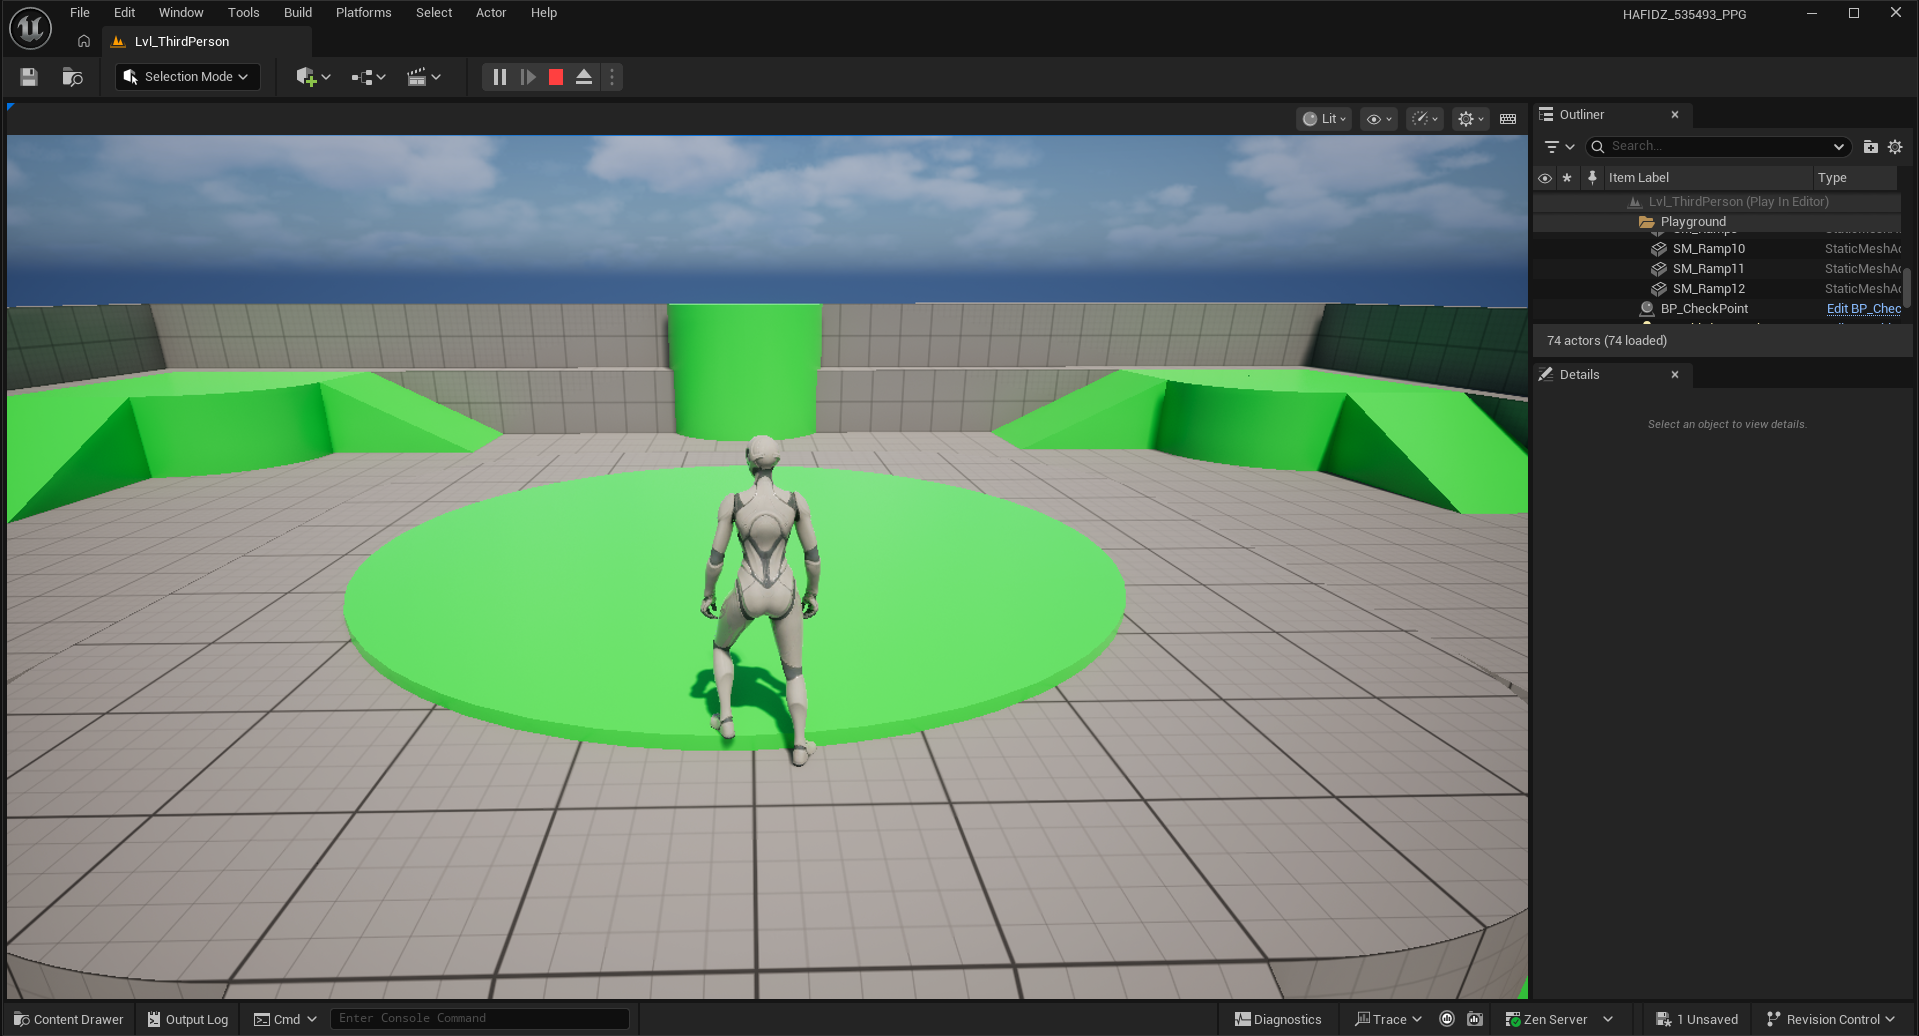
\includegraphics[width=0.9\textwidth]{images/ss-16-hasil-akhir-trigger-checkpoint.png}}
    \caption{Karakter berjalan melintasi BP\_CheckPoint dan memicu penyimpanan data posisi pemain.}
    \label{fig:hasil-trigger-checkpoint}
\end{figure}

Tahap kedua pengujian dilakukan untuk memverifikasi kemampuan pemulihan data simpanan (\textit{persistence}). Simulasi permainan dihentikan dengan menekan tombol \textbf{Stop}, kemudian tombol \textbf{Play} ditekan kembali untuk memulai sesi permainan baru. Saat inisialisasi berjalan, Game Instance mengeksekusi \texttt{Event Init} dan memuat isi berkas slot \texttt{"1"} ke dalam memori. Ketika level dimuat, node \texttt{Event BeginPlay} pada \texttt{BP\_ThirdPersonCharacter} meminta data posisi via \texttt{Get Game Data}. Karena koordinat yang tersimpan bukan bernilai nol, node \texttt{Set Actor Location} memindahkan karakter langsung ke titik koordinat checkpoint terakhir. Karakter berhasil berdiri di lokasi checkpoint tersebut tanpa harus mengulang dari titik \texttt{PlayerStart}, membuktikan integrasi Game Instance dan SaveGame telah berjalan sesuai instruksi modul praktikum \cite{modul5}.

\begin{figure}[H]
    \centering
    \customfbox{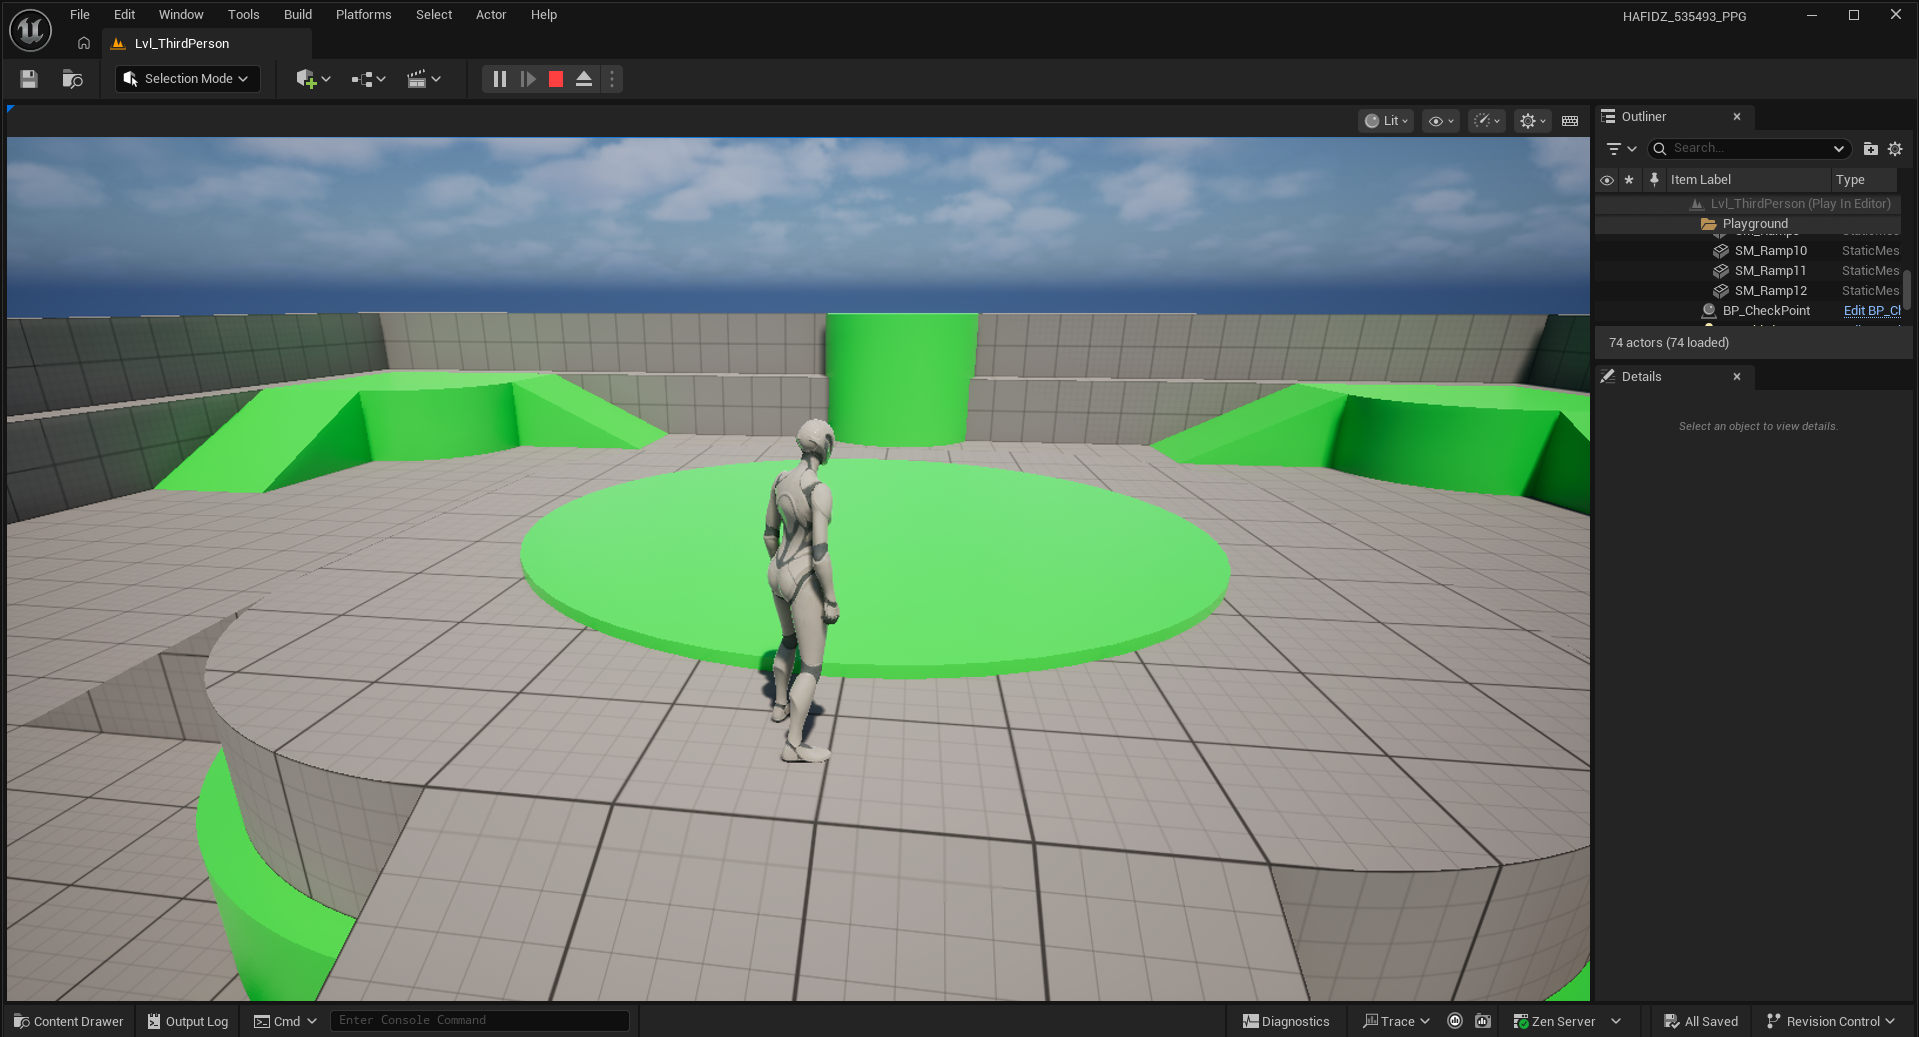
\includegraphics[width=0.9\textwidth]{images/ss-17-hasil-akhir-restore-position-on-play.png}}
    \caption{Hasil uji coba play ulang: karakter otomatis dimuat pada posisi checkpoint terakhir dari berkas SaveGame.}
    \label{fig:hasil-restore-position}
\end{figure}

\clearpage

\chapter{Kesimpulan}
Dari praktikum Pertemuan 5 mengenai Game Instance dan SaveGame ini, saya memahami bagaimana Unreal Engine mengelola data persisten yang melintasi siklus hidup level maupun sesi aplikasi game. Kelas \texttt{BP\_GameInstance} menjadi wadah penyimpan data global yang aman karena tetap berada di memori RAM selama permainan berjalan, berbeda dengan aktor level yang dihancurkan setiap kali peta dimuat ulang.

Penggunaan kelas dasar \texttt{BP\_SaveGame} dan struktur data \texttt{S\_PlayerState} memberikan alur penyimpanan yang rapi. Mengelompokkan koordinat lokasi, rotasi, dan skala ke dalam satu variabel Transform menyederhanakan kabel graph Blueprint. Pengecekan awal dengan node \texttt{Does Save Game Exist} juga mencegah terjadinya galat saat membaca slot berkas penyimpanan yang belum ada. Selain itu, pemanfaatan operasi asinkron terbukti menjaga jalannya game tetap mulus tanpa jeda pembekuan frame saat menulis berkas ke media penyimpanan.

Penerapan antarmuka \texttt{BPI\_SaveData} pada Game Instance kembali memperkuat arsitektur modular tanpa ketergantungan casting langsung. Aktor pemicu \texttt{BP\_CheckPoint} dan karakter pemain dapat saling bertukar data simpanan melalui fungsi pesan antarmuka secara bersih. Hasil pengujian menunjukkan bahwa posisi karakter di checkpoint berhasil ditulis ke berkas lokal \texttt{1.sav} dan langsung dipulihkan saat permainan dijalankan ulang, membuktikan seluruh mekanisme telah bekerja sesuai panduan modul praktikum \cite{modul5}.

\clearpage
\addcontentsline{toc}{chapter}{Daftar Pustaka}
\renewcommand{\bibname}{Daftar Pustaka}
\begin{spacing}{1.05}
\begin{thebibliography}{99}
    \setlength{\itemsep}{0.15em}
    \bibitem{modul5} Modul Praktikum Pengembangan Game Pertemuan 5: Game Instance \& SaveGame, T.A. 2026/2027. Semester Gasal, Universitas Gadjah Mada.
    \bibitem{epic-gameinstance} Epic Games, ``GameInstance in Unreal Engine'', 2026. [Online]. Tersedia: \url{https://dev.epicgames.com/documentation/en-us/unreal-engine/game-instance-in-unreal-engine}.
    \bibitem{epic-savegame} Epic Games, ``Saving and Loading your Game in Unreal Engine'', 2026. [Online]. Tersedia: \url{https://dev.epicgames.com/documentation/en-us/unreal-engine/saving-and-loading-your-game-in-unreal-engine}.
    \bibitem{epic-interface} Epic Games, ``Blueprint Interface in Unreal Engine'', 2026. [Online]. Tersedia: \url{https://dev.epicgames.com/documentation/en-us/unreal-engine/blueprint-interface-in-unreal-engine}.
    \bibitem{epic-structs} Epic Games, ``Structs in Unreal Engine'', 2026. [Online]. Tersedia: \url{https://dev.epicgames.com/documentation/en-us/unreal-engine/structs-in-unreal-engine}.
    \bibitem{epic-collision} Epic Games, ``Collision in Unreal Engine'', 2026. [Online]. Tersedia: \url{https://dev.epicgames.com/documentation/en-us/unreal-engine/collision-in-unreal-engine}.
    \bibitem{epic-naming} Epic Games, ``Recommended Asset Naming Conventions in Unreal Engine Projects'', 2026. [Online]. Tersedia: \url{https://dev.epicgames.com/documentation/en-us/unreal-engine/recommended-asset-naming-conventions-in-unreal-engine-projects}.
    \bibitem{epic-forum-lifecycle} Unreal Engine Community Forum, ``How to check which Begin Play or something similar goes first'', 2024. [Online]. Tersedia: \url{https://forums.unrealengine.com/t/how-to-check-which-begin-play-or-something-similar-goes-first-c/1565114/2}.
    \bibitem{epic-async} Epic Games, ``Asynchronous Loading in Unreal Engine'', 2026. [Online]. Tersedia: \url{https://dev.epicgames.com/documentation/en-us/unreal-engine/asynchronous-loading-in-unreal-engine}.
    \bibitem{yt-savegame} Smart Poly, ``UE5 Save Game Explained Simply'', 2023. [Online Video]. Tersedia: \url{https://www.youtube.com/watch?v=b6Oz6fb_mI0}.
\end{thebibliography}
\end{spacing}

\end{document}
